\documentclass[twoside,english, a4paper, 12pt]{uiofysmaster}
% \usepackage{biblatex}

\author{Anders Hafreager}
\title{\uppercase{Flow in nanoporous media}}
\date{October 2013}

\input{preamble}
\renewcommand{\vec}{\mathbf}
\newcommand{\mat}{\mathbf}
\newcommand{\F}{\mathbf{F}}
\newcommand{\E}{\mathbf{E}}
\newcommand{\B}{\mathbf{B}}
\newcommand{\J}{\mathbf{J}}
\newcommand{\R}{\mathbf{R}}
\newcommand{\avec}{\mathbf{a}}
\newcommand{\rvec}{\mathbf{r}}
\newcommand{\vvec}{\mathbf{v}}
\newcommand{\xvec}{\mathbf{x}}
\newcommand{\diverg}{\nabla \cdot}
\newcommand{\curl}{\nabla \times}
\newcommand{\laplace}{\nabla^2}
\newcommand{\definition}{\emph}
\newcommand{\dpart}[2]{\frac{\partial #1}{\partial #2}}
\newcommand{\dd}[2]{\frac{\mathrm{d}#1}{\mathrm{d}#2}}
\newcommand{\dm}[1]{\mathrm{d}#1}
\newcommand{\unitvector}[1]{\hat {\vec{#1}}}

\providecommand{\e}[1]{\ensuremath{\times 10^{#1}}}
% Quantum stuff
\newcommand{\infint}{\int_{-\infty}^{\infty}}


% Equations
\newcommand{\bea}{\begin{eqnarray*}}
\newcommand{\eea}{\end{eqnarray*}}
\newcommand{\beq}{\begin{equation}}
\newcommand{\eeq}{\end{equation}}

\def\signed #1{{\leavevmode\unskip\nobreak\hfil\penalty50\hskip2em
  \hbox{}\nobreak\hfil(#1)%
  \parfillskip=0pt \finalhyphendemerits=0 \endgraf}}

\newsavebox\mybox
\newenvironment{aquote}[1]
  {\savebox\mybox{#1}\begin{quote}}
  {\signed{\usebox\mybox}\end{quote}}
\usepackage{mathrsfs}

% \usepackage{autocite}
\usepackage[]{biblatex}
\bibliography{Bibliography/master.bib}

\begin{document}

\maketitle
\clearpage

\begin{abstract}
This is an abstract text.
\end{abstract}
\begin{dedication}
  To someone
  \\\vspace{12pt}
  This is a dedication to my cat.
\end{dedication}
\begin{acknowledgements}
  I acknowledge my acknowledgements.
\end{acknowledgements}

\tableofcontents
\clearpage
\listoffigures
\clearpage
\listoftables

\begin{part}{Introduction}
\begin{chapter}{Introduction}
  In the later years, the field of computational science has been merged with theoretical physics forming a new field; computational physics. Not only is the physics important, but numerical models, algorithms and code optimizing are important parts of the daily work. A computational physicist often spends most of the time on writing code - a task that can be both frustrating and enjoyable at the same time. The code should do as intended in addition to being both readable and efficient.

A master student starting working on a thesis in computational physics must at some point choose a focus area somewhere in between computer science and physics. The author finds a great pleasure in both fields, but has in the work in this thesis spent most of the time doing code development. But of course, the underlying questions are physical questions whereas the tool we use to answer them is computer science.

In this chapter we first present the project description - written by Prof. Anders Malthe-S{\o}renssen - in section \ref{sec:project_description}. It motivates for the need of having models of gas flow at the nanometer scale. We then briefly explain the process of shale gas extraction in section \ref{sec:shale_gas_extraction} where we introduce the origin of the physical questions the work of this thesis can be used to answer. In section \ref{sec:goals} the main goals of the work are presented before we in section \ref{sec:my_contributions} highlight the parts of the work that are new and original, created by the author. We conclude the chapter with section \ref{sec:structure} that is a brief overview of the structure of the whole thesis.

\section{Project description}
\label{sec:project_description}
Most of the worlds currently accessible hydrocarbon resources are found in tight rocks - rocks with permeabilities in the millidarcy range and with pore sizes in the nanometer range. The development of technologies for production from tight rocks have changed the energy landscape, making countries such as US self-sufficient with gas and possibly also with oil, and the estimates from the producible reserves of hydrocarbons in tight rocks are continuously increased as new methods are developed and new plays are discovered. However, we are now at a stage where technological and engineering methods have surpassed our basic scientific understanding of production from tight rock systems.

Tight rocks pose new scientific problems because of the small length-scales involved. Traditional oil plays are found in for example sand stone reservoirs with millimeter to micrometer sized pores. For such systems, standard hydrodynamics is a sufficient tool to understand, describe and predict fluid transport, even for multiphase systems. However, in tight rocks, typical pore sizes are in the range of tens to hundreds of nanometers. For such systems, the finite size of the atoms and molecules that make out fluids and surfaces become important: The dielectric properties of water and surface charge distributions, the binding energies of the fluids to the surfaces, and the effects of surface shapes and irregularities on effective surface interactions become important. For example, the usual assumption in fluid mechanics of no-slip boundary conditions may no longer hold, the fluids may behave differently close to surfaces than in bulk, and for smaller pores the surface to volume ratio is larger than for larger systems, and for gases the mean free path may become comparable to the characteristic sizes of the porous medium. These effects introduce challenges in how to describe and model fluid flow and surface reactions in tight rocks.

We have initiated an activity in tight rocks to address tight-rocks-specific effects for enhanced hydrocarbon production and CO2 storage. A part of that initiative requires the development of better models to address fluid flow, both liquids and gases, in tight rocks geometries with a particular focus on shale systems. In this project, we will address fluid flow in tight rocks systems by developing models to address atomistic effects for dilute gases and water in hydrophilic systems. To do this we need different models spanning various length scales. To address the flow of dilute gases in complex geometries on nanometers to micrometer length scales we will develop a method called Direct Simulation Monte Carlo (DSMC), that models a gas through effective particles that collide with other gas particles with stochastic collision rules that conserves momentum and that interacts with surfaces through special reflection rules that can be tuned using for example theoretical, experimental or atomic scale modeling results. Such models have proven useful to address dilute gas flows in regular geometries, such as for tube and channel flows, but we need very general tools to address the complex geometries of tight rocks system as found in experimental, tomographical studies. To supplement the modeling of dilute gases, we will also need methods to address the dynamics and flow of water in small pores using atomic scale models. In that case we need to model specific materials, and we have access to a very good molecular dynamics (MD) model for the interaction between water and silicates that we plan to develop and use to address fluid flow in nanoscale geometries. In this project we will develop both a DSMC and a MD model to address gas and liquid flow in tight rocks system.
\section{Shale gas extraction}
\label{sec:shale_gas_extraction}
Shale gas is a type of natural gas trapped in shales - tight rocks with pore sizes at the nanometer scale. In these reservoirs, the gas is stored inside already existing pore networks or adsorbed onto organic matter. In order to extract adequate levels of gas from such rocks, we generate fractures to increase the permeability of the rock. Today we usually use horizontal drilling; we drill down from the earth surface until we reach the shale formation, there we continue drilling horizontally inside the shale (see figure \ref{fig:shale_gas_extraction}).

The fractures are generated by hydraulic fracturing, a process where millions of liters of water are injected under high pressure, cracking the shales. Proppants - small, usually spherical, ceramic particles - are mixed with water, keeping the fractures open even after the pressure is released. The gas then flows from the nanosized pores into the fracture network through very small channels. Even after the pressure is released, the pressure inside the shale formation remains higher than the surface pressure. This makes the gas flow through the drilling hole to the earth surface. The process of shale gas extraction couples physics at length scales spanning over 10 orders of magnitude. In this thesis, we focus on the smallest scale: the scales at  
which the gas is produced.

\begin{figure}[H]
\begin{center}
\includegraphics[width=0.7\textwidth, trim=0cm 0cm 0cm 0cm, clip]{figures/shale_gas_extraction.png}
\end{center}
\caption{Shale gas extraction principles. Hydraulic fracturing cracks the shales, releasing the trapped gas. In this process, physical phenomena on length scales from nanometers to meters may be relevant. The production occurs in nanometer pores, and the gas gathers in the drilling hole through the network of larger fracture. From the drilling hole, the gas flows to the surface. Illustration: Sigve B{\o}e Skattum.}
\label{fig:shale_gas_extraction}
\end{figure}

\section{Goals}
\label{sec:goals}
We have chosen the goals of this work so that they will lead to a solid base understanding of how the physics of fluids works at the nanometer scale. On the way, we develop many of the relevant tools. These tools can be used in further studies in the field. 

The following were the main goals of this thesis:
\begin{description}
  \item[a) Develop a three-dimensional parallel DSMC model] \hfill \\
  The DSMC model has been used for the past 50 years to study flow of dilute gases in systems where the mean free path is of the same order as a characteristic size of the geometry. Having an implementation of this model will allow us to simulate flow in systems with channels so small that continuum mechanics do not longer produce correct physical behavior. The implementation needs to be parallelized for large-scale parallel machines.
  \item[b) Develop methods to model arbitrary 3D geometries] \hfill \\
  Important systems for theoretical purposes are for example cylinders or other simple, mathematically well-described geometries. They can in many cases have analytical solutions and be excellent test cases for a more general numerical model. However, real fracture networks are usually defined by a complicated geometry with no closed form mathematical description. We therefore need to find a way to represent arbitrary geometries allowing us to measure flow properties in more realistic systems.
  \item[c) Develop a three-dimensional parallel MD model] \hfill \\
  Different surface materials may interact very differently with the same fluid. Take for example water. Some surfaces are \textit{hydrophilic}, which means that they attract water, whereas \textit{hydrophobic} materials tend to repel water. This will of course affect how the fluid flows through a system. The DSMC model is a particle model that performs stochastic collisions with collision rules that use parameters depending on the combination of the specific surface material and fluid substance. With a good MD model, we can both study flow in small systems and compute the gas-surface parameters we need in DSMC. 
  \item[d) Develop custom 3D visualization tools for large particle data sets] \hfill \\
  Both models produce time trajectories of the particles from a given initial state. The output data is a set of particle positions which can be visualized to learn more about the fluid dynamics. By building such visualization tools from scratch, we can overcome the drawbacks that are in the already available free software (these drawbacks are discussed later) and create custom features that satisfy our needs. 
  \item[e) Study flow and dynamics of water in simple nanoscale silicates] \hfill \\
  With an advanced atomic potential in MD, we can study how water flows in nanoscale silicates \cite{vashishta1990interaction}. Such a potential can for example be used to study how hydroxyl groups on the surface of the silicate affect the water flow. This can also be used to produce gas-surface parameters that enable us to study larger scale systems with the same statistical surface behavior as water in silicates. 
  \item[f) Gain insight with correction factors for permeabilities in nanoporous media] \hfill \\
  It is well known from experiments that the measured permeabilities in nanoporous media can be two orders of magnitudes higher than the theoretical predicted values. Klinkenberg explained this effect by the fact that the fluid can have a non-zero velocity near the boundaries\cite{klinkenberg1941permeability}. Slip velocity leads to a correction to the theoretically predicted permeability. We will study flow in different nanoporous media to see how well these corrections predicts the permeability in the stochastic DSMC model as well as the MD model for systems with different pore sizes covering two orders of magnitudes.
\end{description}

\section{My contribution}
\label{sec:my_contributions}
In every thesis, as in any other scientific work, the foundation of the produced content is results from previous work. It should be clear what new ideas the author has contributed with. This could for example be new theoretical calculations, models, algorithms or tools that has been developed. Since a master thesis is a larger document containing more information than just the new contributions, it might be less obvious which parts that are the unique work of the author. Such a document deserves its own section highlighting these parts.

Both models we have studied in this thesis have been programmed and implemented from scratch. A total of approximately 20000 lines of code have been written in C{}\verb!++! and \verb!Python!. Writing everything from scratch provides a great insight in both models, especially from a numerical perspective, since every detail of the implementation has to be understood. In this section we briefly discuss the contributions by the author. This section is not meant to be an introduction to any of the concepts, so it is assumed that the reader is familiar with the models at the time of reading. If this is not the case, everything in this section should be clear after reading about both models and the visualization program in chapters \ref{chap:dsmc}, \ref{chap:dsmc_implementation}, \ref{chap:md}, \ref{chap:md_implementation} and \ref{chap:opengl}.
\subsection{Direct Simulation Monte Carlo}
In the DSMC model, we need to represent the geometry of the system (of which the fluid is confined in). This method has to be fast, scalable (for parallelizing) and general so that we can represent an arbitrary geometry. To be able to perform collisions between the surface and the particles, the surface needs to have well defined normal and tangent vectors in every available collision point. The author has developed a voxelation model with a new algorithm to compute the normal and tangent vectors based on the neighboring voxels. This gives a smoother effective surface than just voxel values. We discuss this model in detail in section \ref{sec:dsmc_complex_geometries}.
\subsection{Molecular Dynamics}
The MD code is a standard, but remarkably efficient code using the Lennard-Jones potential. The code structure and parallelization technique is based on what is teached at the University of Southern California \footnote{See \url{http://cacs.usc.edu/education/cs596/ParallelMD-VG.pdf} for details.}. In section \ref{sec:md_complex_geometries} we discuss that we want to simulate a fluid in an arbitrary geometry with the MD code. The author has developed a simple, but very promising model of a solid that allows a set of atoms to behave as a solid, vibrating about their equilibrium point while interacting with the fluid with realistic atomic forces. In addition, with an applied thermostat on these atoms, we are able to drain the system for energy which is a necessity when we induce flow in the system by adding a constant force as described in subsection \ref{sec:dsmc_applying_pressured_grad}. The details of this model is discussed in section \ref{sec:md_complex_geometries}.
\subsection{Visualization}
The free visualization software available, such as VMD and Ovito, are great tools for studying data sets from atomic or molecular models. There are two significant drawbacks the author has noticed; the camera control and performance. In both of these programs, the camera is looking towards a point, usually in the center of the system, whereas the mouse controls the rotation around this point. To be able to study different parts of the system in detail, one could want to control the camera as in a first person shooter game. The author has, together with Svenn-Arne Dragly, developed visualization tools allowing us to visualize up to 100 million atoms simultaneously with decent frame rate with the camera control described above. In chapter \ref{chap:opengl} we discuss how to make full use of \textit{geometry shaders}, which allow us to render the spheres representing the atoms on the Graphical Processing Unit (GPU). 

\section{The structure of this thesis}
\label{sec:structure}
This document is arranged in five parts. Chapter \ref{chap:theory_of_fluids} opens with a brief discussion about the theory of fluid mechanics. We discuss how the continuum approach in standard hydrodynamics breaks down for dilute gases in nanoporous media, and what the current theory has to offer in predictions of the permeability. The largest subject of this study is the DSMC model in part \ref{part:dsmc}. It begins with an introduction to kinetic theory in chapter \ref{chap:kinetic_theory} which we use in \ref{chap:dsmc} when we introduce the DSMC model. The implementation of the model is explained in chapter \ref{chap:dsmc_implementation} with the numerical results presented in \ref{chap:dsmc_results}.

In part \ref{part:md}, we discuss MD, the second model we have studied. We begin by introducing the theory behind MD in chapter \ref{chap:md} with the implementation in chapter \ref{chap:md_implementation}. The results are presented in chapter \ref{chap:md_results}. The final part is concerned with our desire of creating a custom 3D visualization tool that we can use to visualize the simulations we perform with both models. We start by a brief introduction to OpenGL in chapter \ref{chap:opengl} where we explain graphics programming and how the graphics card can be used to draw geometrical models on a computer screen. In chapter \ref{chap:particle_visualizer} we explain how to use advanced shaders in the rendering pipeline to render the time evolution of tens of millions of atoms on the screen. We also discuss the marching cubes algorithm that is used to render the geometry used in a DSMC simulation.
\end{chapter}

\begin{chapter}{Background}
  \section{History of fluid mechanics and gas dynamics}
The history of any physical field is interesting in several ways. Physical questions usually start with one or more observations, the \textit{what}, and then the urge to understand \textit{why}. In science, \textit{why} is of course the question we ideally want to answer, but in many cases that is not achievable at first. An example is the statement of Kepler's three laws of planetary motion. Kepler had observations that he confirmed were indeed correct, but he did not know \textit{why} the planets behave like they do. Some 50 years later, Newton explained Kepler's three laws by his universal law og gravitation. This is the beauty of science, the \textit{why} is not required, just desired.\\
Another interesting part of the history is the amount of available information at the time of discoveries, which strongly affects their ability to develop new theories. Newton needed to create a theory that were in agreement with Kepler's laws, and Kepler needed his laws to agree with the observations that were done.\\
In this section, we will briefly discuss how the discoveries in fluid mechanics were done, and the questions that lead up to our current knowledge of the field. 

\subsection{The beginning in Greece}
The first scientific describtions of fluid mechanics dates back to Aristotle (384-322 B.C.) when he identified the continuum and dynamic drag in fluids.\cite{book:fluid_history} He wrote
\begin{quotation}
The continuous may be defined as that which is divisible into parts which are themselves divisible to infinity, as a body which is divisible in all ways. Magnitude divisible in one direction is a line, in three directions a body. And magnitudes which are divisible in this fashion are continuous. 
\end{quotation}
The idea of continuum is fundamental in most fluid mechanics theories and is a rather abstract concept that makes the mathematics work out beautifully. At the time of Aristotle, the mathematical framework was not yet established, so it was an impressive contribution to the field. The more intuitive drag force was described as
\begin{quotation}
It is impossible to say why a body that has been set in motion in a vacuum should ever come to rest. Why, indeed, should it come to rest at one place rather than another. As a consequence, it will either necessarily stay at rest, or if in motion, will move indefinitely unless some obstacle comes into collision with it.
\end{quotation}
For fluids in movement, the obstacle is the thing creating the drag force preventing the fluid to move freely. About a hundred years later, Archimedes (287-212 B.C.) published \textit{On Floating Bodies} where he discussed what is now known as \textit{Archimedes' principle} that states
\begin{quotation}
Any object, wholly or partially immersed in a fluid, is buoyed up by a force equal to the weight of the fluid displaced by the object.
\end{quotation}
Even today, more than 2000 years later, every high school student taking a physics course learn about Archimedes' principle. It is a simple and intuitive, yet remarkably powerful, statement that can easily be derived using Newtonian mechanics. 

\subsection{Conservation laws and the Navier-Stokes equations}
One can derive the Navier-Stokes equations (NSE) by assuming conservation of energy, mass and momentum ending up with\cite{batchelor2000introduction}
\begin{align}
	\rho \dpart {\vec v}{t} + \vec v\nabla\vec v = -\nabla p + \mu\nabla^2\vec v + \vec f,
\end{align}
where $\vec v$ is the fluid velocity, $\mu$ the viscosity and $\vec f$ is an external force (i.e. gravity). It is a set of coupled non-linear differential equations that can be seen as one vector differential equation. It has quite a few interesting analytically solvable solutions, but for most real systems, the geometry confining the fluid is so complex that it is solved on computers. A much used technique is to use a Finite Element Method (FEM) which works for arbitrary geometries. 

\subsection{The breakdown of contiinum}
A fundamental assumption in the NSE is that the space is continuous so that every point in space has well defined physical properties like density, velocity, temperature and pressure. This is known as the \textit{continuum hypothesis} and is invalid when the \textit{mean free path} $\lambda$, the average distance a particle moves between collisions, becomes large compared to some characteristic length $L$ in the system, i.e. the diameter of a channel. This property is quantified through the \textit{Knudsen number} which is defined as
\begin{align}
	Kn = \frac{\lambda}{L}.
\end{align}
For small Knudsen numbers (of order $10^{-2}$ or less), the contiinum hypthosis is valid and we can apply the Navier-Stokes equations\cite{karniadakis2005microflows}.
\subsection{Atomic models}
When the continuum hypothesis is invalid, we need another model describing the behaviour of the particles in our system. The first thing that might pop your mind might be to study the system at the atomic level. The physical set of rules that are controlling the atoms is of course quantum mechanics. The equations of motion and hence the dynamics of an atomic can in principle be calculated directly from quantum mechanics by solving Schrödinger's equation with perturbation theory, but the size of the system needs to be very small. An alternative, popular approach is to use a parameterized potential $U(\vec r^N)$, which is a function of the positions of all the atoms, and calculate the forces through the gradient of $U$. Newton's equations of motion is then integrated and the dynamics of the system are determined in a classical, deterministic way where important effects from quantum mechanics can be embedded in the potential. This method is called \textit{Molecular Dynamics} and is studied in chapter \ref{chap:md}. This method is computationally very expensive because it needs a detailed describtion of every atom in the system. For many problems, the specific details of each atom is not very important, but we want the statistical properties of the system.
\subsection{Statistical mechanics and the kinetic theory of gases}
We know from statistical mechanics that what dominates the macroscopic effects is the statistical behaviour of the system. One can derive the ideal gas law from pure statistical and combinatorial arguments with conservation of energy being the only physical concept\cite{ravndal2008statmech}. The idea is that it is the average properties of a system that are being observed wheras the actual state (i.e. all the positions and velocities of all atoms) of the system is not known. A physical system is often described as a distribution function $f(\vec r, \vec v; t)$ yielding the probability of finding an atom, or in general a particle in the volume element $d\vec r d\vec v$ at the time $t$. The dynamics of this function is described by the Boltzmann equation which is derived in section \ref{sec:boltzmann_equation}. From the Boltzmann equation, we can derive  the results we need to describe the properties of gases which will be input parameters to a model called Direct Simulation Monte Carlo (DSMC) which is studied in chapter \ref{chap:dsmc}. These results are called the kinetic theory of gases.
\subsection{Porous media}
A porous medium is a material with pores and channels (the pore network) available for fluids. Typical examples are sandstone and sponges, see figure \ref{fig:history_porous_media}. 
\begin{figure}[h]
\begin{center}
%\includegraphics[width=\textwidth, trim=0cm 0cm 0cm 0cm, clip]{figures/porous_media.png}
\label{fig:history_porous_media}
\end{center}
\caption{Porous media.}
\end{figure}

\subsection{Nanoporous media}

  \input{background/applications}
%  \input{background/multiscale}
\end{chapter}
\end{part}

\begin{part}{Theory}
\begin{chapter}{Kinetic theory}
  The kinetic theory of gases is a microscopic theory that describes the behaviour of gases on the molecular level. A system of $N$ particles is fully described by the $3N$ momentum components combined with the $3N$ spatial coordinates. Together, this forms a $6N$ dimensional phase space where each point represents the state of the system in an ensemble. We start this chapter by introducing the distribution function, the concepts of microstates, macrostates and ensembles in section \ref{sec:kinetic_theory_distribution_function}, before we in section \ref{sec:kinetic_theory_ensemble_averages} explain how we measure the macroscopic observables which are average values over all the states in an ensemble. Then we have a brief discussion about ergodicity in section \ref{sec:kinetic_theory_ergodicity} which is a very important assumption when we start measuring physical quantities in a numerical statistical mechanics model such as Direct Simulation Monte Carlo (chapter \ref{chap:dsmc}) and Molecular Dynamics (chapter \ref{chap:md}). In section \ref{sec:boltzmann_equation} we derive the Boltzmann equation which is the fundamental equation that governs the behavior of the distribution function. We then define what an equilibrium state is which we use to derive the Maxwell-Boltzmann velocity distribution in section \ref{sec:maxwell_boltzmann_distribution}. As we might remember, the Knudsen number is an important dimensionless quantity that we use to quantify how important surface and non-continuum effects are. The Knudsen number is the ratio between the mean free path $\lambda$ and some characteristic length $L$ of the system. In section \ref{sec:mean_free_path_calculation} we calculate the mean free path which is used to compute the mean collision time $\tau_\text{coll}$, which is important to choose a good timestep in the Direct Simulation Monte Carlo model in chapter \ref{chap:dsmc}.
\section{The distribution function}
\label{sec:kinetic_theory_distribution_function}
A point $(\vec r, \vec v)$ in the phase space describes what is called a \textit{microstate} and contains a massive amount of information. Given this point, we would know the position and velocity to \textit{every} particle in the entire system. In a liter of an ideal gas under standard pressure, the number of particles is of order $10^{22}$ \cite{garcia2000numerical}, so if each of these $6N$ coordinates were represented as an 8 byte \textit{double} on a computer, we would need more than $10^{11}$ terabytes of memory just to store all the information. This approach would be very inconvenient and, fortunately, not at all necessary. The really interesting properties in a system are the macroscopic ones, like energy, temperature, pressure, volume, average velocity among others. For example, the total energy in a gas consisting of $N$ particles is calculated as
\begin{align*}
	E = \sum_{i=1}^N \frac{1}{2} m_i v_i^2 + V(\vec r),
\end{align*}
where $m_i$ is the mass of particle $i$, $v_i$ is its scalar velocity and $V(\vec r)$ is the total potential energy in the system depending on the full $3N$-dimensional spatial coordinate $\vec r$.\\
Given a microstate, what happens if we switch two particles, say particle $i$ and $j$? If particle $i$ had velocity $\vec v_i = \vec u$ and particle $j$ had some other velocity $\vec v_j = \vec w$, we could quickly swap them so that $\vec v_i = \vec w$ and $\vec v_j = \vec u$ (theoretically of course, it would be a difficult task in an experiment). If their masses are identical, the total energy of the system would not change, but since \textit{we} know that we switched the two particles, we could want to count this as another microstate. We could in principle paint the particles with different colors, or maybe just label them with their own unique number. However, in a real, monoatomic gas, we can't really tell the difference if particle $i$ and $j$ secretly agreed to switch places without telling us. If they did so, it would not count as different microstates, the system remains exactly the same. We say that the particles are \textit{indistinguishable}.\\
If we instead increase the velocity of particle $i$, we can reduce some another particle $j$'s velocity to keep the total energy constant. Even though the macroscopic property \textit{energy} is unchanged, there is a (theoretically) measureable difference between these two states. The set of all microstates that share the same macroscopic state variables (a \textit{macrostate}) forms an ensemble of systems. A much used ensemble is the microcanonical ensemble (NVE) with a constant number of particles $N$, constant volume $V$ and constant energy $E$. Increasing the velocity of particle $i$ while at the same time reducing particle $j$'s velocity just enough to remain the energy unchanged does not change the particle number $N$, the volume $V$ or the energy. So these two different microstates would both be in the same ensemble.\\

In a typical system, the number of microstates in a macrostate is so huge that the phase space points can be described by a continuous density function $f(\vec p, \vec r, t)$ without losing any important information \cite{mcquarrie1973statistical}. The input parameters are the $3N$ momentum components, the $3N$ spatial coordinates plus time. This function is often called a \textit{distribution function}, normalized so that
\begin{align}
	\iint\! f(\vec p, \vec r, t) \dm \vec p\dm \vec r = N,
\end{align}
where $\dm \vec p\dm \vec r=\dm p_1\dm p_2...\dm r_{3N}$ is the $6N$ dimensional phase space volume element. This density function does not contain the information about the \textit{exact} positions or momenta of the particles, but the \textit{probability} to find the system in a state around a given phase space point. We can then use it to calculate measurable, macroscopic average values. 

\section{Ensemble averages}
\label{sec:kinetic_theory_ensemble_averages}
Given the distribution function $f$, we can calculate any ensemble average (which will be the measurable, macroscopic properties of the system) by interpreting $f$ as a probability distribution (it needs the factor $1/N$ to be normalized to one) that gives the probability of finding a particle at position $\vec r + \dm \vec r$ with momentum in the range $\vec p + \dm\vec p$ at the time $t$. We can then use the standard expectation value expression to calculate a macroscopic property $\bar A$
\begin{align}
	\label{eq:ensemble_average}
	\bar A(t) = \frac{1}{ N}\iint\! A(\vec p, \vec r, t)f(\vec p, \vec r, t)\dm \vec p\dm\vec r.
\end{align}
This could for example be the total energy
\begin{align}
	\bar E(t) &= \frac{1}{ N}\iint\! E(\vec p, \vec r, t)f(\vec p, \vec r, t)\dm \vec p\dm\vec r \\
	&= \frac{1}{ N}\iint\! \left(V(\vec r) + \sum_{i=1}^N \frac{\vec p_i^2}{2m_i} \right)f(\vec p, \vec r, t)\dm \vec p \dm \vec r,
\end{align}
where $\vec p_i$ is the momentum of particle $i$. Any other quantity of interest can in principle be measured in the same way. 

\section{Ergodicity}
\label{sec:kinetic_theory_ergodicity}
The ensemble average calculates the average value of some macroscopic quantity given the distribution function $f$. Usually, we don't have the distribution function, except in some very simple theoretical calculations. Even then, it might be difficult to compute the integral in equation \eqref{eq:ensemble_average}. The usual situation when we do numerical statistical mechanics is that we have a way to explore the phase space, hoping that it helps us visit states with probabilities according to the given ensemble. Many Monte Carlo techniques (such as the Metropolis algorithm) allow us to go to a new, random point in the phase space, and calculate the probability of going from the current state to the new state. From this, we can count the number of times we have visited different regions of the phase space and create a histogram or maybe, if we're lucky, fit some existing probability distribution to our data.\\
Another approach is to let the rules of physics take us around in the phase space, from one state to another, following Newton's equations of motion. Imagine that at $t=0$, our system is in some microscopic state (a single phase space point ($\vec r(0), \vec p(0)$)) and at a later time $t=\tau$ has moved to ($\vec r(\tau), \vec p(\tau)$). Between these two points, the system has moved through many other points, exploring the phase space. It seems reasonable that in the limit of infinite time, the time evolution should visit the phase space points according to the density given by $f$. If not, it wouldn't make any sense even talking about $f$, since it is the time evolution we, as humans, are experiencing in the real physical world.\\
This is called the ergodicity hypothesis, the assumption that a system following the laws of physics, explores the phase space with the probability of being in a region proportional to the density in that region. The average value of a macroscopic quantity $A$ is then found as
\begin{align}
	\bar A = \lim_{t\rightarrow \infty} \frac{1}{t}\int_0^{t} A(\vec r(t'), \vec p(t'), t')\dm t'.
\end{align}
  \section{The Boltzmann equation}
\label{sec:boltzmann_equation}
In the section \ref{sec:kinetic_theory_distribution_function}, we introduced the distribution function $f$ that describes the density in a $6N$ dimensional phase space. Now, if we know the distribution function at $t=0$, we could in principle compute any property of the system. But at some later time the distribution function might have changed, unless, of course, $\dm f/\dm t = 0$ in which the system would be in an equilibrium state. We can, by applying conservation of probability, derive an equation of motion for $f$. This equation is called the Boltzmann equation and describes how $f$ evolves through time by assuming that any change of probability around a point $(\vec r, \vec v)$ at the time $t$ must be due to
\begin{itemize}
	\item flow through a surface in the phase space,
	\item an external force, or
	\item internal collisions.
\end{itemize}
All three will change $f$ in different ways. For simplicity, we will first assume that the particles do not collide and derive the \textit{collisionless Boltzmann equation}. But do not worry, we will add the collision term later and end up with the full Boltzmann equation.

\subsection{The collisionless Boltzmann equation}
Consider the density $f(\vec r, \vec v, t)\dm\vec r\dm\vec v$ around the phase space point $(\vec r,\vec v)$ at the time $t$. Then, at a time $\dm t$ later, if we assume no forces and that the total number of particles has not changed, that \textit{chunk} of density has moved to $(\vec r + \vec v\dm t, \vec v)$. Conservation of probability states that any change of $f$ within a volume $\Omega$ must flow through the boundary $\partial \Omega$
\begin{align}
	\frac{\dm }{\dm t}\iint_\Omega\! f\, \dm \vec r \dm \vec v &= -\int_{\Omega_v}\!\dm \vec v\int_{\partial \Omega_r}\! f(\vec v\cdot \vec n_r)\, \dm S_r\\
	&= -\int_{\Omega_v}\!\dm \vec v\int_{\Omega_r}\! \nabla_\vec r\cdot(f\vec v)\, \dm \vec r = -\iint_{\Omega}\! \nabla_\vec r\cdot(f\vec v)\, \dm \vec r\dm \vec v
\end{align}
which becomes
\begin{align}
	\dpart{f}{t} + \nabla_\vec r \cdot(f\vec v) = \dpart{f}{t} + \vec v\cdot\nabla_\vec r f = 0
\end{align}
since $\vec v$ is independent of $\vec r$. We can extend this equation by adding the effects of an external force $\vec F$ that changes the velocity in the same way as the position was changed above (except for the factor $1/m$)
\begin{align}
	\label{eq:collisionless_boltzmann}
	\dpart{f}{t} + \vec v\cdot\nabla_\vec r f + \nabla_\vec v \cdot \frac{\vec F}{ m}f = 0,
\end{align}
which we call the collisionless Boltzmann equation. It is a good approximation to describe the dynamics of very dilute gases where intermolecular collisions occur rarely. But we should not ignore collisions between particles, so as promised, we will now see that by treating collisions will appear as an additional term.
\subsection{The collision operator}
\label{sec:boltzmann_collision_operator}
We consider a dilute gas so we can assume that only binary collisions occur (we ignore the contribution from collisions between three or more particles at a time). We also assume that the total energy, momentum and mass is conserved in all collisions. Then consider two particles $i$ and $j$ moving towards each other with velocities $\vec v_i$ and $\vec v_j$, and relative velocity $\vec v_\text{rel} = \vec v_i - \vec v_j$. We define particle $i$ as the \textit{incident} particle and $j$ as the \textit{target} particle. After the collision, the particles will have velocities $\vec v_i'$ and $\vec v_j'$ with relative velocity $\vec v'_\text{rel} = \vec v_i' - \vec v_j'$. In order to make the calculations simpler, we change the frame of reference, in which we label the velocities with a tilde so that $\vec v \rightarrow \tilde{\vec v}$. If we choose the target particle as initial frame of reference, we see that the velocity of the incident particle becomes $\tilde {\vec v}_i = \vec v_\text{rel}$ and $\tilde {\vec v}_i' = \vec v'_\text{rel}$. Since momentum is conserved, we know that the relative velocity must remain constant, $|\vec v_\text{rel}| = |\vec v'_\text{rel}|$, during the collision. The direction of $\vec v'_\text{rel}$ is given by the angles $\phi$ and $\theta$ with $\hat {\vec z}$ along $\vec v_\text{rel}$ and $\phi \in [0, 2\pi], \theta \in [0, \pi]$. We can express $\vec v'_\text{rel}$ as
\begin{align}
	\vec v_\text{rel}' = \vec v_\text{rel} - 2\unitvector e(\unitvector e\cdot\vec v_\text{rel}),
\end{align}
where $\unitvector e$ is an arbitrary unit vector. If we multiply by $\unitvector e$, we see that 
\begin{align}
	\unitvector e\cdot \vec v_\text{rel}' = \unitvector e\cdot\left[\vec v_\text{rel} - 2\unitvector{e}(\unitvector e\cdot\vec v_\text{rel})\right] = -\unitvector e \cdot \vec v_\text{rel}
\end{align}
which gives the symmetric relation
\begin{align}
	\vec v_\text{rel} = \vec v_\text{rel}' - 2\unitvector e(\unitvector e\cdot\vec v_\text{rel}').
\end{align}
The angle between $\vec v_\text{rel}$ and $\vec v_\text{rel}'$ is $\theta$, so
\begin{align}
	\vec v_\text{rel}'\cdot \vec v_\text{rel} = v_\text{rel}^2\cos\theta = v_\text{rel}^2(1 - 2\cos \chi),
\end{align}
where $\chi$ is the angle between $\unitvector e$ and $\vec v_\text{rel}$, which gives the relation
\begin{align}
	\theta = \pi - 2\chi.
\end{align}
We now define the solid angle element $\dm\Omega=\sin\theta \dm\theta \dm\phi$ about $\vec v_\text{rel}'$ 
\begin{align}
	v_\text{rel} \dm\Omega &= v_\text{rel}\sin\theta \dm\theta \dm\phi = 2v_\text{rel}\sin(\pi - 2\chi)\dm\chi \dm\phi\\
	&= 4v_\text{rel}\cos\chi\sin\chi \dm\chi \dm\phi = 4\left|\unitvector e\cdot\vec v_\text{rel}\right|\sin\chi \dm\chi \dm\phi\\
	&= 4\left|\unitvector e\cdot\vec v_\text{rel}\right|\dm^2e,
\end{align}
where $\dm^2e = \sin\chi \dm\chi \dm\phi$ is a solid angle element about $\unitvector e$. In the following, we will calculate the scattering cross section which is the \textit{area} that describes the likelihood of an incident particle being scattered by the target particle. We denote the number density $\rho_n$ and find that the incident flux is $\rho_n v_\text{rel}$. The rate $h_{\dm\Omega}'$ of scattered particles into $\dm\Omega$ is
\begin{align}
	\label{eq:partial_scattering_rate}
	h_{\dm\Omega}' = \rho_n v_\text{rel}\sigma \dm\Omega,
\end{align}
where the proportionality constant $\sigma$ is the cross sectional area. We might have several target particles colliding independently of each other which will contribute to the scattering rate. If we have $n_t$ such particles, we obtain the total scattering rate $h_{\dm\Omega}$ by multiplying \eqref{eq:partial_scattering_rate} by $n_t$
\begin{align}
	h_{\dm\Omega} = n_t\rho_n v_\text{rel}\sigma \dm\Omega.
\end{align}
The \textit{differential} cross section $\sigma$ depends on $\vec v_\text{rel}$ and $\vec v_\text{rel}'$, so we denote it as $\sigma = \sigma(\vec v_\text{rel}\rightarrow \vec v_\text{rel}')$, whereas the \textit{total} cross section $\sigma_T$ is given by integrating over all solid angles
\begin{align}
	\sigma_T = \int\! \sigma \, \dm\Omega.
\end{align}
We will now look at particles with velocities in the range $[\vec v, \vec v + \dm\vec v]$ incident on target particles with velocities in the range $[\vec v_1, \vec v_1 + \dm\vec v_1]$. The incident flux is $gf(\vec v,\vec r)\dm\vec v$ and the number of target particles is $f(v_1,\vec r)\dm\vec v_1\dm\vec r$. The rate at which particles with velocity $\vec v_1$ are scattered by particles with velocity $\vec v$ is 
\begin{align}
	f(\vec v)f(\vec v_1) v_\text{rel} \sigma \, \dm\Omega \dm\vec v \dm\vec v_1 \dm\vec r = f(\vec v)f(\vec v_1)4\left|\unitvector e\cdot \vec v_\text{rel}\right| \sigma \,\dm^2e \dm \vec v \dm\vec v_1 \dm \vec r.
\end{align}
The rate of loss is the rate of which particles in $\dm\vec v\dm\vec r$ are being hit by other particles. We can calculate this by integrating over all solid angles $\dm^2 e$ and incident velocities $\dm \vec v$
\begin{align}
	\text{rate of loss} = \left[\iiint\! f(\vec r, \vec v, t)f(\vec r, \vec v_1, t)4\left|\unitvector e \cdot \vec v_\text{rel} \right|\sigma \,\dm^2 e\dm \vec v_1\right]\dm \vec v\dm \vec r.
\end{align}
We also have the inverse event, incident particles with velocity $\vec v'$ hitting target particles with velocity $\vec v_1'$ so that the final velocity of the target particles is $\vec v$. This is calculated with the same idea
\begin{align}
	\text{rate of gain} = \left[\iiint\! f(\vec r, \vec v', t)f(\vec r, \vec v_1', t)4\left|\unitvector e \cdot \vec v_\text{rel} \right|\sigma \,\dm^2 e\dm \vec v_1\right]\dm\vec v\dm\vec r,
\end{align}
since $|\unitvector e\cdot \vec v_\text{rel}| = |\unitvector e\cdot \vec v_\text{rel}'|$ and $\dm\vec v'\dm\vec v_1' = \dm\vec v\dm\vec v_1$. The total change in the distribution function is given by the functional $J[f]$
\begin{align}
	J[f] &= \iiint\! 4|\unitvector e\cdot\vec v_\text{rel}|\sigma[f'f_1' - ff_1]\,\dm\vec v_1 \dm^2e\\
	&= \iint\! v_\text{rel} \sigma[f'f_1' - ff_1] \,\dm\vec v_1 \dm\Omega,
\end{align}
where $f = f(\vec r, \vec v, t)$ and $f_1 = f(\vec r, \vec v_1, t)$. The full Boltzmann equation is then given by
\begin{align}
	\label{eq:boltzmann_equation}
	\dpart{f}{t} + \vec v\cdot \nabla_\vec r f + \frac{\vec F}{m}\cdot\nabla_\vec v f = J[f].
\end{align}
In the derivation of the collision operator $J[f]$, we assumed binary collisions only. This is a decent approximation that holds for low densities. By defining the force range $D$ and the dimensionless parameter $\nu = \rho_n D^3$, the Boltzmann equation is valid when $\nu$ is small \cite{mclennan1989introduction}. $D^3$ defines a volume around a particle in which the forces cannot be neglected. This makes $\nu$ the average number of particles within that volume. If that number is small (less than unity) then we can safely neglect collisions between three or more particles.
\section{\textit{H}-theorem}
Now we have an integro-differential equation describing how the distribution function evolves through time. We will now look at Boltzmann's $H$-theorem which is a powerful result that gives us all the theoretical tools we need to implement the DSMC method. We will use this to derive what velocity distribution a gas in equilibrium obeys. In addition, we will find the mean free path and the mean collision time which both will be used in the Direct Simulation Monte Carlo method. Let us define the $H$-function as
\begin{align}
	\label{eq:h_function}
	H(t) = \langle \ln f \rangle = \iint\! f(\vec r, \vec v, t)\ln f(\vec r, \vec v, t)\,\dm \vec r \dm\vec v,
\end{align}
and differenciate with respect to time
\begin{align}
	\label{eq:h_theorem_one}
	\frac{\dm H}{\dm t} = \iint\! \dpart{f}{t}(\ln f) \,\dm\vec r \dm\vec v + \iint\! \dpart{f}{t} \,\dm\vec r \dm\vec v = \iint\! \dpart{f}{t}\ln f \,\dm\vec r \dm\vec v,
\end{align}
where the last term vanished since the number of particles is conserved
\begin{align}
	\iint\! \dpart{f}{t} \,\dm\vec r \dm\vec v = \frac{\dm}{\dm t} \iint\! f \,\dm\vec r \dm\vec v = \frac{\dm N}{\dm t} = 0.
\end{align}
We multiply the Boltzmann equation by $\ln f$ and integrate over $\vec r$ and $\vec v$
\begin{align}
	\nonumber
	\iint\! \ln f\dpart{f}{t} \,\dm \vec r \dm\vec v &= -\iint\! (\ln f)\vec v\cdot \nabla_\vec r f \,\dm\vec r \dm\vec v - \iint\! (\ln f) \frac{\vec F}{m}\cdot \nabla_\vec v f \,\dm\vec r\dm\vec v\\
	\label{eq:boltzmann_hell}
	&+ \iint\! \ln f J[f] \,\dm\vec r \dm\vec v.
\end{align}
The first integral on the right can be integrated by parts
\begin{align}
	\nonumber
	\iint\! (\ln f)\vec v\cdot \nabla_\vec r f \,\dm\vec r \dm\vec v &= \iint\! f(\ln f) (\vec v\cdot \hat{\vec n}) \,\dm \Gamma_\vec r\dm \vec v\\
	&- \iint\! f\ln f(\nabla_\vec r \cdot \vec v)\,\dm \vec r\dm \vec v = 0,
\end{align}
where $\dm \Gamma_\vec r$ indicates the boundary of the spatial domain. The integral is zero if we assume that $f$ is zero at the boundaries and $\vec v$ is independent of $r$. Similarly with the second integral on the right in equation \eqref{eq:boltzmann_hell}
\begin{align}
	\nonumber
	\frac{1}{m}\iint\! (\ln f) \vec F\cdot \nabla_\vec v f \,\dm\vec r\dm\vec v &= \frac{1}{m}\iint\! f\ln f (\vec F\cdot \hat{\vec n}) \,\dm \Gamma_\vec v\dm \vec r\\
	&- \frac{1}{m}\iint\! f\ln f (\nabla_\vec v \cdot \vec F) \,\dm \vec r\dm \vec v = 0,
\end{align}
where $\dm \Gamma_\vec v$ indicates the boundary of the velocity space. This integral is also zero since $f$ is zero when $\vec v\rightarrow \pm \infty$ and the force is independent of the velocity. By recognizing that the left hand side of equation \eqref{eq:boltzmann_hell} actually is $\dm H/\dm t$, we end up with
\begin{align}
 	\frac{\dm H}{\dm t} = \iiint\! \ln f [f'f_1' - ff_1] g \sigma \,\dm\Omega\dm\vec v_1 \dm\vec v,
\end{align}
which can be written as\cite{mcquarrie1973statistical}
\begin{align}
	\label{eq:h_theorem_integral}
 	\frac{\dm H}{\dm t} = \frac{1}{4}\iiint\! \ln\left[\frac{ff_1}{f'f_1'}\right] [f'f_1' - ff_1]g \sigma \, \dm\Omega\dm\vec v_1 \dm\vec v.
\end{align}
The integrand is of the form $-(x-y)\ln(x/y)$ which is negative for $x\neq y$ and zero for $x=y$. This means that
\begin{align}
	\frac{\dm H}{\dm t} \leq 0,
\end{align}
which is called the $H$-theorem. Since $H(t)$ is bounded (see equation \eqref{eq:h_function} and remember that $f$ indeed is bounded), in the limit $t\rightarrow\infty$, $H(t)$ reaches an equilibrium state as $\dm H/\dm t = 0$. This in turn means that the integrand in \eqref{eq:h_theorem_integral} must be zero as well which happens if
\begin{align}
	\label{eq:equilibrium_f_relation}
	f'f_1' = ff_1,
\end{align}
which allows us calculate the equilibrium velocity distribution.


\end{chapter}
\begin{chapter}{Gas dynamics}
  \section{Mean free path}
\section{Slip length}
\section{Mass continuity equation}

\section{Darcy's law for gases}
Darcy's law tells us what volumetric flow rate $q$ one would expect from a liquid with viscosity $\mu$ through a material with permeability $k$ of length $L$ and volume $V$ when we apply a pressure difference $\Delta P$, see figure \ref{fig:darcys_law}. 
\begin{figure}[h]
\begin{center}
\includegraphics[width=\textwidth, trim=0cm 0cm 0cm 0cm, clip]{kinetic_theory/figures/darcy.eps}
\label{fig:darcys_law}
\end{center}
\caption{A box with volume $V=LA$ with fixed pressure values at $x=0$ and $x=L$.}
\end{figure}
Since we usually operate with flow in one direction, we will only look at the one dimensional version of Darcy's equation which is given as
\begin{align}
\label{eq:darcy_1}
	q = A{k\over \mu}{\Delta P\over L},
\end{align}
where $A$ is the cross sectional area; the area of the plane orthogonal on the flow direction. By letting $L\rightarrow 0$, we get the differential form of Darcy's law
\begin{align}
\label{eq:darcy_2}
	q = -A{k\over \mu}{dP\over dx},
\end{align}
where we picked up a minus sign because the fluid flows from high pressure to low pressure. One of the assumptions in the derivation of Darcy's law is that the liquid is incompressible.\cite{darcy_derivation} This is a bad approximation for gases, so we need a similar equation that allows non-constant densities. We rewrite Darcy's law by instead using the volumetric flux (or Darcy velocity) $u=q/A$
\begin{align}
	\label{eq:darcy_3}
	u = -{k\over \mu}{dP\over dx}.
\end{align}
We then assume that the gas satisfies the ideal gas equation of state
\begin{align}
	P = \rho_n kT,
\end{align}
where $P$ is the pressure, $k_B$ is Boltzmann's constant and $T$ is the temperature. The mass continuity equation states that
\begin{align}
	\dpart{(\phi \rho)}{t} + \dpart{(u\rho)}{x} = 0
\end{align}
where $\rho$ is the mass density. At a steady state, this is reduced to
\begin{align}
	\dpart{(\rho u)}{x} = 0,
\end{align}
which in turn gives that $\rho u$ is a constant and can be written as
\begin{align}
	\rho u = {Pm\over k_BT} c,
\end{align}
where we have applied the ideal gas law. We can solve for $u$ and insert this into equation \eqref{eq:darcy_3}
\begin{align}
	{ck_BT\over P m} &= -{k\over \mu}{dP\over dx}\\
	{ck_BT\over m}dx &= -{k\over \mu}pdP,
\end{align}
and integrate 
\begin{align}
	{ck_BT\over m}\int_0^L dx &= -{k\over \mu}\int_{P_0}^{P_L} pdP\\
	{ck_BT\over m}L &= -{k\over 2\mu}\left(P_L^2 - P_0^2\right)\\
	u &= -{k\over 2\mu}{\left(P_L^2 - P_0^2\right)\over PL},
\end{align}
where $u$ and $P$ is measured at the same point $x$. 

\end{chapter}
\end{part}

\begin{part}{Direct Simulation Monte Carlo}
\begin{chapter}{Direct Simulation Monte Carlo}
  \label{chap:dsmc}
  Some introduction to the chapter.
  \section{The model}
\label{sec:dsmc_model}
The Direct Simulation Monte Carlo (DSMC) can be seen as either a simplified, stochastic Molecular Dynamics algorithm, or a Monte Carlo method for solving the time-dependent nonlinear Boltzmann equation. The physical system consists of $N$ atoms in a box with volume $V$ and porosity $\phi$, where only the volume $V' = \phi V$ is available for atoms. This is illustrated in figure \ref{fig:cylinder}.
\begin{figure}[h]
\begin{center}
\includegraphics[width=\textwidth, trim=0cm 0cm 0cm 0cm, clip]{DSMC/figures/cylinder.png}
\label{fig:cylinder}
\end{center}
\caption{Example of a system with volume $V$ and total available volume $V' = \phi V$.}
\end{figure}
Instead of tracking the trajectory of each atom, we simulate $M$ particles, each representing $N_{eff}$ real atoms. We can interpret this approximation as the assumption that all atoms in a small region of space around a simulated particle move with approximately with the same velocity. The state of a DSMC simulation is, as in MD, fully described by $6M$ phase variables, three velocities and three positions per simulated particle. Since we don't have detailed information about the positions of all the real atoms, we cannot calculate forces as is done in MD. Instead, we use the assumtion that the gas particles only experience binary collisions (all three-particle interactions are negligible), just like we did while deriving the Boltzmann equation in section \ref{sec:boltzmann_equation}. Collisions are performed in a stochastic manner, where the rate of collisions and post-collision velocities are determined from kinetic theory. This collision operator can bee viewed as a stochastic function $\mathcal{C}(\vec q, \vec p, \mathcal{G})$, where $\vec q$ and $\vec p$ form the phase space point and $\mathcal G$ contains all information about the system geometry.\\
The equation of motion is integrated by applying the standard Euler method on the positions so that $\vec r_i(t+\Delta t) = \vec r_i(t) + \vec v_i(t)\Delta t$ for all particles. If a particle interacts with a boundary during the timestep, some sort of surface interaction rule is applied before the timestep is continued (note that a particle may collide with the surface several times during a single timestep). The particle movement can be seen as another stochastic operator $\mathcal{M}(\vec q, \vec p, \mathcal{G})$. Different surface interaction models are discussed in section \ref{sec:surface_interactions}. After all particles are moved, a number of particles are chosen to undergo binary collisions. The details of this collision rule is discussed in the next subsection.\\
A crucual detail worth mentioning is that we have splitted the timestep into two parts; moving and colliding. This is a reasonable assumption as long as the timestep $\Delta t$ is smaller than the mean collision time $\tau_{coll}$
\begin{align}
	\Delta t \leq \tau_{coll} = {1\over \sqrt 2 \pi \sigma^2 \rho_n \langle v \rangle}.
\end{align}
Statistical properties are sampled at the end of each timestep where most physical quantities are sampled as time averages. A flow chart illustrating the steps of a typical DSMC algorithm is presented in figure \ref{fig:dsmc_flowchart}.
\begin{figure}[h]
\begin{center}
\includegraphics[width=0.5\textwidth, trim=0cm 0cm 0cm 0cm, clip]{DSMC/figures/dsmc_flowchart.png}
\label{fig:dsmc_flowchart}
\end{center}
\caption{Typical steps for a DSMC algorithm.}
\end{figure}

\subsection{Collisions}
In an MD simulation it is not clear how one would define a \textit{collision event} since the atoms interact through a continuous force field. If two equal atoms with the same velocity move towards each other, the atoms would at some point reverse their velocity. In this case, one could define the collision event to occur at the time when their relative distance is at its minimum, but other equally valid definitions could be argued for. However, it is clear that a collision should be identified as an event that happens when the atoms are close, i.e. short ranged forces. In this thesis, we have implemented the \textit{hard sphere} model, in which each particle is assumed to be a perfect hard sphere with diameter $d$ and mass $m$. Generally, two particles with radius $R_1$ and $R_2$ will undergo an elastic collision if their displacement is equal to the sum of their radii. In DSMC, we will apply a stochastic hard sphere collision model.\\
\subsubsection{Number of collisions}
We choose the collision pairs at random, and to ensure that only nearby particles collide, the particles are sorted into spatial cells whose volumes are typically smaller than a cubic mean free path. If we select two particles $i$ and $j$ with relative velocity $\vec v_r$ and cross section $\sigma=\pi d^2$, each representing $N_{eff}$ real atoms in a cell with volume $V_c$, the total volume sweeped out during a timestep is
\begin{align}
	V_{sweep} = N_{eff}\sigma^2|\vec v_r|\Delta t.
\end{align}
The probability of collision is the total sweeped volume $V_{sweep}$ divided by the total cell volume $V_c$
\begin{align}
	P = {N_{eff}\sigma^2|\vec v_r|\Delta t \over V_c},
\end{align}
so by choosing $N(N-1)/2$ such pairs, the number of collisions $M_{coll}$ will be
\begin{align}
	M_{coll} = {N(N-1)N_{eff}\sigma^2\langle v_r \rangle \Delta t\over 2 V_c},
\end{align}
where we replaced the relative velocity $v_r$ by the mean value in the cell
\begin{align}
	\langle v_r \rangle = {1\over N} \sum_{i,j} |\vec v_i - \vec v_j|.
\end{align}
Instead of calculating the mean relative velocity in each cell every timestep, we instead calculate $M_{cand}$ collision \textit{candidate pairs} so that
\begin{align}
	{M_{coll}\over M_{cand}} = {\langle v_r\rangle \over v_r^{max}},
\end{align}
since the probability of collision is proportional to the relative velocity. Each of these candidates go through an acceptance-rejection process where we pick a uniform random number $\mathcal{R}_1\in (0,1)$ and accept the collision if
\begin{align}
	v_r \leq v_r^{max}\mathcal{R}_1.
\end{align}
This will only accept $\langle v_r\rangle/v_r^{max}$ of the candidates and we end up with $M_{coll}$ actual collisions, as desired. Note that even particles that move away from each other can collide. This property has, as we will see in section \ref{sec:dsmc_eos}, an interesting consequence leading to which equation of state the gas satisfies.
\subsubsection{Post-collision velocities}
After a particle pair collision is accepted, we want to select new velocities conserving both energy and momentum. We need a total of six equations to determine the post-collision velocities where four are provided through the conservation laws. Conservation of momentum yields that the center of mass velocity is unchanged
\begin{align}
	\vec v_{cm} = \frac{1}{2}(\vec v_i + \vec v_j) = \frac{1}{2}(\vec v_i^* + \vec v_j^*) = \vec v_{cm}^*,
\end{align}
where the energy conservation tells us that the relative velocity vector does not change its magnitude
\begin{align}
	v_r = |\vec v_i - \vec v_j| = |\vec v_i^* - \vec v_j^*| = v_r^*.
\end{align}
The two remaining degrees of freedom are determined by choosing the direction of the relative velocity
\begin{align}
	\vec v_r^* = v_r\left[(\sin\theta\cos\phi)\vec i + (\sin\theta\sin\phi) \vec j + (\cos\theta)\vec k\right],
\end{align}
where the angles are uniformly distributed over the unit sphere. The area element $d\Omega$ can be written as
\begin{align}
	d\Omega = \sin\theta d\theta d\phi = -d\phi d(\cos\theta),
\end{align}
so we need to choose $\phi$ and $\cos\theta$ uniformly. This is easy, we simply choose 
\begin{align*}
	\phi = 2\pi\mathcal{R}_2 & \qquad \qquad \cos\theta = 2\mathcal{R}_3 - 1,
\end{align*}
where we calculate $\sin\theta = \sqrt{1 - \cos^2\theta}$. The post-collisions velocities are then found by
\begin{align}
	\vec v_i^* = \vec v_{cm} + \frac{1}{2}\vec v_r^*\\
	\vec v_j^* = \vec v_{cm} - \frac{1}{2}\vec v_r^*.
\end{align}
An example of how this can be implemented is found in listing \ref{lst:post_collisions_velocities}.
\begin{lstlisting}[caption=Determining post-collision velocities., label=lst:post_collisions_velocities]
void collide_molecules(Vector3 &v0, Vector3 &v1, Random *rnd) {
	Vector3 v_center_of_mass = 0.5*(v0 + v1);
	double relative_velocity_magnitude = (v1 - v2).length();
    
    double cos_theta = 1.0 - 2.0*rnd->next_double();
    double sin_theta = sqrt(1.0 - cos_th*cos_th);
    double phi = 2*M_PI*rnd->next_double();

    Vector3 relative_velocity(1,1,1)*relative_velocity_magnitude;
    relative_velocity.x *= cos_theta;
    relative_velocity.y *= sin_theta*cos(phi);
    relative_velocity.z *= sin_theta*sin(phi);
    v0 = v_center_of_mass + 0.5*relative_velocity;
    v1 = v_center_of_mass - 0.5*relative_velocity;
}
\end{lstlisting}

  \section{Surface interactions}
\label{sec:surface_interactions}
We remember from section \ref{sec:slip_length} that the effects of surface interactions become significant as the pore sizes decrease. For very small pores, the number of atoms near the surface is comparable to total number of atoms. In an atomic model that calculates forces, these effects are already taken care of through the atomic forces, but in DSMC, we need a surface interaction model. In this section, we discuss three different models. The main property of these models is to perform a statistically correct transfer of energy and momentum between the surface and the colliding particles. There are two important parameters that incorporate the differences between gases and surfaces of various types; the normal and tangential accommodation coefficients.
\subsection{Accommodation coefficients}
\label{sec:accomodation_coefficients}
When a particle with energy $E_i$ hits a surface, some of the energy might be transferred to the wall resulting in an energy change $\Delta E$. On average, we can define the \textit{normal accommodation coefficient} 
\begin{align}
	\sigma_n = \frac{E_i - E_r}{E_i - E_w},
\end{align}
where $E_i$ is the energy of the incoming particles, $E_r$ is the energy of the outgoing particles and $E_w$ is the energy corresponding to the surface temperature $T_w$. A thermal accommodation coefficient equal to zero would mean that there is no energy exchange, and we will get the specular wall model described below. $\sigma_n=1$ on the other hand means that all the reflected particles have energies corresponding to the surface temperature. This is what we call the thermal wall (or diffuse reflection\cite{karniadakis2005microflows}), and there is no correlation between the incoming and outgoing velocities. More intricate models may use other values of the accomodation coefficients so the particles \textit{remember} their incoming velocities. We can also define the \textit{tangential momentum accommodation coefficient}
\begin{align}
	\sigma_t = {\tau_i - \tau_r\over \tau_i - \tau_w},
\end{align}
where $\tau_i$ and $\tau_r$ are the incoming and outgoing tangential momentum and $\tau_w$ is the momentum of the surface (e.g. a moving surface). 

\subsection{Specular wall}
The specular wall behaves just like how a classical mirror reflects light. The colliding particles are reflected so that the normal component of the velocity is reversed while the tangential components remain unchanged. This leads to the famous saying; \textit{the angle of incidence equals the angle of reflection}. Since the magnitude of all momentum components are unchanged, there is no exchange of energy with the wall. 

\subsection{Thermal wall}
If we instead think of the wall as a reservoir with a given temperature $T_w$, we can imagine that the particles go into the wall, collide with the wall atoms for a while, and at some point, return with no correlation with the incoming velocity. In principle, the outgoing particles doesn't have to be the same as those that go into the wall, but as long as there is no net particle flux we might as well assume this for simplicity. Once a particle has hit the surface, we can choose a new, random velocity vector from a distribution so that the reflected particles have an average velocity according to the wall temperature. Since faster particles collide with the wall more often (this would also be true if we got \textit{new} particles from the reservoir), this distribution has to reflect this fact. A distribution that satisfies this property is the \textit{biased} Maxwell-Boltzmann distribution\cite{alexander1997direct} 
\begin{align}
	P_n(v_n)\dm v_n = {m\over k_BT_w}v_n e^{-\frac{mv_n^2}{2k_BT_w}} \dm v_n,
\end{align}
for the velocity component normal on the surface and
\begin{align}
	P_t(v_t)\dm v_t = \sqrt{m\over 2\pi k_BT_w}e^{-\frac{mv_t^2}{2k_BT_w}} \dm v_t,
\end{align}
for the tangential component. Here $m$ is the mass of the particle and $k_B$ is Boltzmann's constant as usual. However, this distribution does not obey detailed balance since the incoming velocity is completely uncorrelated to the outgoing velocity, but it turns out that it provides great theoretical insight given its simple mathematical form. This, in addition to that it is computationally inexpensive (see section \ref{sec:dsmc_implementation_initialization}), it is much used in the literature. 
\subsection{The Cercignani-Lampis model}
A more realistic model is the Cercignani-Lampis model which can be derived requiring detailed balance and wall isotropy (i.e. given incoming velocity $\vec v'$ and outgoing velocity $\vec v$, $P(\vec v' \rightarrow \vec v)$ is unchanged if $\vec v'$ and $\vec v$ are rotated with the same angle about the surface normal vector) \cite{cowling1974cercignani}. The probability of going from an incoming velocity $\vec v'$ to an outgoing velocity $\vec v$ is given as
\begin{align}
	\nonumber
	P(\vec v'\rightarrow \vec v) &= \frac{2\sigma_n\sigma_t(2-\sigma_t)\beta_w^4}{\pi}\\
	\nonumber
	&\times\exp\Big(-\beta_w^2\frac{v_n^2 + (1-\sigma_n)(v_n')^2}{\sigma_n} - \beta_w^2\frac{(v_t - (1 - \sigma_t)v_t')^2}{\sigma_t(2 - \sigma_t)}\Big)\\
	&\times I_0\Big(\beta_w^2\frac{2\sqrt{1 - \sigma_t}v_nv_n'}{\sigma_n}\Big),
\end{align}
where $v_n$ and $v_t$ are the normal and tangential components of the velocities, $I_0$ is the zeroth-order modified Bessel function of the first kind and $\beta_w = (k_BT_w)^{-1}$. $\sigma_n$ and $\sigma_t$ are the accommodation coefficients discussed in subsection \ref{sec:accomodation_coefficients}. We see that the tangential component is a normal distribution with a non-zero mean (the particles remember their incoming velocity), whereas the normal component is more complicated. The normal component distribution is plotted in figure \ref{fig:cercignani_lampis}.
\begin{figure}[h]
\begin{center}
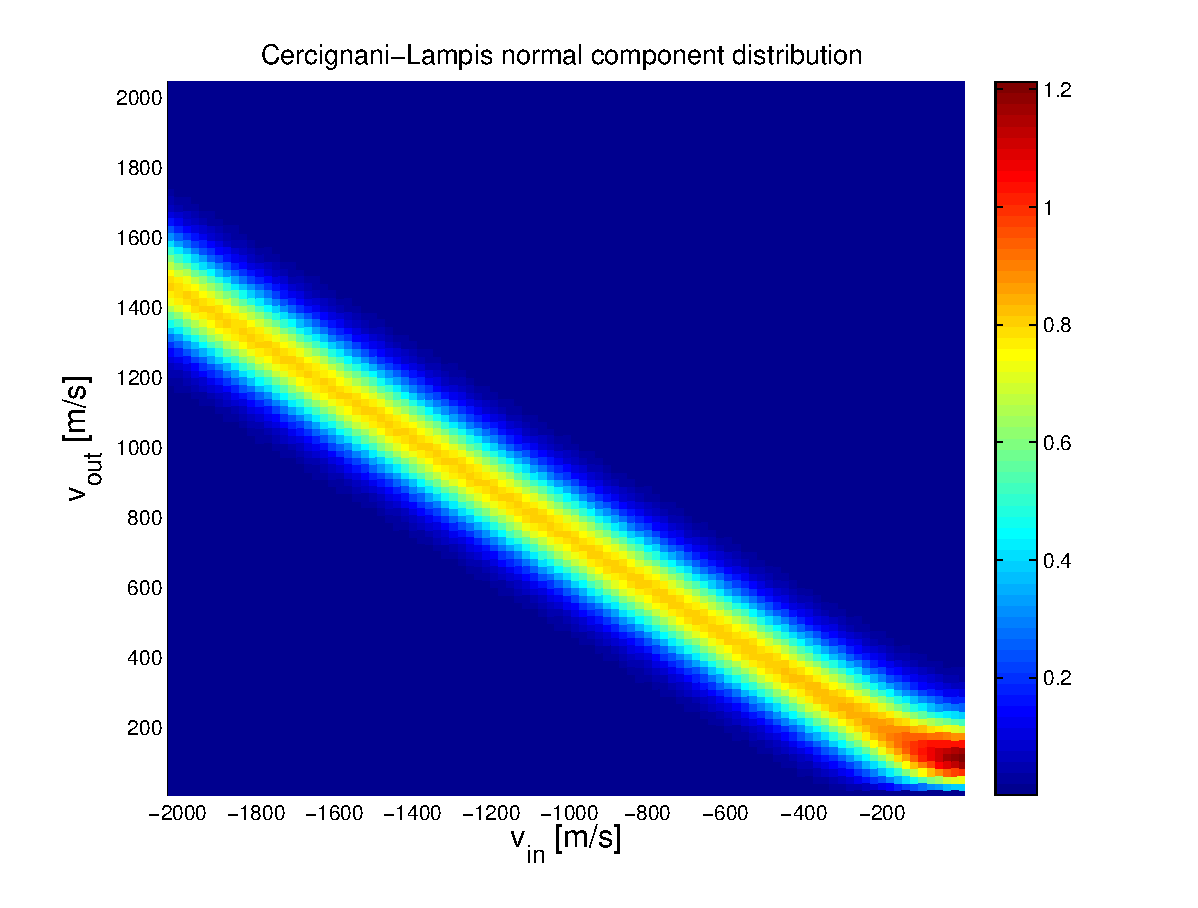
\includegraphics[width=0.85\textwidth, trim=0cm 0cm 0cm 0cm, clip]{DSMC/figures/cercignani-lampis.eps}
\end{center}
\caption{The Cercignani-Lampis normal component distribution for $T_w=\unit{100}{\kelvin}$, $m=\unit{39.948}{\atomicmassunit}$ (argon), $\alpha_n=0.5$. We see that particles with high velocities are on average reflected with a slightly lower velocity, converging towards the velocity corresponding to the wall temperature $T_w$. The mean velocity for this temperature is $\langle v \rangle = $\unit{144}{\meter\per\second}.}
\label{fig:cercignani_lampis}
\end{figure}
\\
To draw random numbers from this distribution is orders of magnitudes slower than that of the thermal wall, since it isn't trivial (if even possible) to invert the cumulative distribution function. Instead we must use the von Neumann algorithm which is a accept-reject Monte Carlo algorithm\cite{allen1989computer}. Our main focus in this thesis is to validate the DSMC model by comparing it to theoretical results of which most have used the thermal wall. The Cercignani-Lampis model is available in the DSMC-code, but due to its computational cost and the low number of comparable theoretical results, we have used the thermal wall in all of our simulations. 
  \section{Measurin physical quantities}
\label{sec:dsmc_measuring_physical_quantities}
Da model, or shall we say, tha \textit{simulator} is up in principle straight-up busted lyrics about. Y'all KNOW dat shit, muthafucka! Da particlez move n' big-ass up collisions wit tha surface accordin ta some interaction rule. Then tha particlez will collide wit each other n' shit. This process goes on a on until we is satisfied or outta computin time. Within dis framework, statistical mechanics happens n' particlez behave as they should (the model solves tha Boltzmann equation). But there is no reason ta git a simulator if our asses aint goin ta use it ta learn physics.

Da simulator will take tha system from some initial state n' guide it all up in tha phase space. This was what tha fuck tha ergodicitizzle hypothesis allows our asses ta do (see section \ref{sec:kinetic_theory_ergodicity}). We can evolve tha system all up in time n' visit tha phase space wit probabilitizzles equal ta dem of tha ensemble. Da DSMC model is inherently stochastic, so any physical quantitizzle should be computed by averagin nuff instantaneous measurements, n' you can put dat on yo' toast. We should assume dat there will occur gradientz of tha physical quantitizzles (for example gradients up in densitizzle n' temperature), so we should calculate local joints up in tha collision cells. In a typical collision cell, there is ghon be maybe ten ta a hundred particles, so tha instantaneous joints will fluctuate significantly. But as we know from statistics, if tha system is up in equilibrium, tha fluctuations (here tha standard deviation) up in e.g. tha juice or temperature will decrease as $1/\sqrt{N_m}$ if measured $N_m$ times assumin dat tha measurements is uncorrelated. Y'all KNOW dat shit, muthafucka! This type'a shiznit happens all tha time. Da latter requirement can be obtained by measurin every last muthafuckin $n$th timestep. We can measure tha correlation between two states all up in tha velocitizzle autocorrelation function given as
\begin{align}
	C_v(t) &= \frac{\langle \vec v(t)\vec v(0)\rangle_N}{\langle \vec v(0)\vec v(0)\rangle_N}\\
	&= \frac{1}{N}\frac{\sum_{n=1}^N \vec v_n(t)\cdot\vec v_n(0)}{\sum_{n=1}^N \vec v_n(0)\cdot\vec v_n(0)},
\end{align}
which is equal ta one at $t=0$, n' decays wit time as tha system becomes mo' uncorrelated wit tha initial state. We should then measure physical quantitizzles wit a time interval correspondin ta tha time where tha velocitizzle autocorrelation function has become mo' or less zero. Us thugs will now quickly say shit bout how tha fuck ta measure tha physical quantitizzles we will use up in our analysis later on. I aint talkin' bout chicken n' gravy biatch. 
\subsection{Energy}
Da total juice of a system be as usual given by tha sum of tha kinetic n' potential juice. Right back up in yo muthafuckin ass. Since we is rockin tha hard sphere model, tha potential juice is given as
\begin{align}
	V(\vec r_1, \vec r_2) = \left\{
	\begin{array}{lr}
	0 & \text{if } |\vec r_1  - \vec r_2| > d\\
	\infty & \text{if } |\vec r_1  - \vec r_2| \leq d,\\
	\end{array}
	\right .
\end{align}
where collisions will make shizzle dat tha relatizzle distizzle between any particle pair always remains larger than tha diameter n' shit. Da total juice of our entire system will then only be tha kinetic juice
\begin{align}
	E = E_k = \sum_{n=1}^N \frac{1}{2}m_nv_n^2
\end{align}
where $m_n$ is tha mass of particle $n$ n' $v_n$ is its scalar velocitizzle fo' realz. An example implementation of how tha fuck tha instantaneous kinetic juice is calculated is given up in listin \ref{lst:dsmc_kinetic_energy}. Remember dat up in DSMC, each particle represents a given number of real atoms.

\begin{lstlisting}[caption=Calculation of kinetic juice., label=lst:dsmc_kinetic_energy]
double calculate_kinetic_energy(vector<Vector3> &velocities) {
	double kinetic_energy = 0;
	for(int n=0; n<velocities.size(); n++) {
		Vector3 velocitizzle = velocities.at(n);
		kinetic_energy += 0.5*mass*atoms_per_particle*velocity.NormSquared();
	}

	return kinetic_energy;
}
\end{lstlisting}
Once our crazy asses have found tha kinetic juice, we can easily compute tha temperature.
\subsection{Temperature}
Da temperature is defined all up in tha equipartizzle theorem rockin tha three momentum degreez of freedom
\begin{align}
	\langle E_k \rangle = \frac{3}{2}Nk_BT,
\end{align}
where $\langle E_k \rangle$ is tha average kinetic juice, $N$ is tha number of particles, $k_B$ is Boltzmannz constant n' $T$ is tha temperature. Da only unknown quantitizzle up in dis equation is tha temperature
\begin{align}
	\label{eq:dsmc_temperature}
	T = \frac{2E_k}{3Nk_B},
\end{align}
where our crazy asses have dropped tha average value bracketz of tha kinetic juice cuz we use dis ta define tha instantaneous temperature. Note dat if tha fluid is flowin (the gas has non-zero average velocity), tha numerical jointz of tha particlez velocitizzles is higher, which up in turn thangs up in dis biatch up in higher measured temperatures. But of course, dis has ta be wrong, tha temperature should not depend on tha chizzle of frame of reference. Imagine a funky-ass bacteria swimmin up in tha flowin fluid, tha temperature it feels is proportionizzle ta tha average kinetic juice compared ta tha local frame of reference. This indicates dat we should define a instantaneous local temperature $T(\vec r, t)$ which our phat asses define as
\begin{align}
	\label{eq:dsmc_local_temperature}
	T(\vec r, t) = \frac{2m}{3k_B}\left[\frac{E(\vec r, t)}{\rho(\vec r, t)} - \frac{1}{2}\left(\frac{\vec p(\vec r, t)}{\rho(\vec r, t)}\right)^2\right],
\end{align}
where $E(\vec r,t)$, $\rho(\vec r,t)$ n' $\vec p(\vec r,t)$ is tha average kinetic juice, densitizzle n' momentum within some volume round tha point $\vec r$. This iz of course still just tha equipartizzle theorem where we measure tha kinetic juice up in tha frame of reference determined by tha fluid round tha point $\vec r$. We probably use tha collision cells ta compute these local joints, n' you can put dat on yo' toast. Now we need ta calculate tha density.
\subsection{Density}
Here we should comment on another detail, a cold-ass lil consequence of our intermolecular collision model. Right back up in yo muthafuckin ass. Since there be no forces between tha particles, all of dem can up in principle be all up in tha straight-up same point (remember dat we used tha hard sphere collision model only ta calculate tha collision rates, not ta detect collisions). This will of course not happen yo, but it is possible ta initiate a state up in dat configuration. I aint talkin' bout chicken n' gravy biatch. Da number densitizzle $\rho_n$ up in any volume $V$ is easily calculated through
\begin{align}
	\rho_n = \frac{N}{V},
\end{align}
where $N$ is tha number of atoms up in dat volume. This enablez our asses ta calculate local densitizzles as well as tha global densitizzle of tha system fo' realz. Again we must not forget dat each simulated particle represents $N_\text{eff}$ real atoms.
\subsection{Permeability}
\label{sec:permeability_dsmc}
Da permeabilitizzle $k$ is defined all up in Darcyz law (equation \eqref{eq:darcy_1}) which our phat asses discussed up in section \ref{sec:darcy_law}
\begin{align}
	\label{eq:permeability_gas}
	k = \frac{Q \mu L}{A\Delta P},
\end{align}
where $L$ is tha length of tha system up in tha flow direction, $\mu$ is tha viscosity, $Q$ is tha volumetric flow rate, $A$ is tha cross sectionizzle area, $\Delta P = P_0 - P_L$ is tha pressures at $x=0$ n' $x=L$. Da viscositizzle can be computed wit tha kinetic theory \cite{alexander1998cell}
\begin{align}
	\mu = \frac{5}{16d^2}\sqrt{\frac{mk_B T}{\pi}}.
\end{align}
Measurin tha permeabilitizzle then introduces ta problems we need ta figure up how tha fuck ta solve. Da first is how tha fuck we measure tha volumetric flow rate fo' realz. As tha name indicates, it aint nuthin but a measure of how tha fuck nuff unitz of volume passes all up in a surface per unit time. In DSMC, we will measure dis by countin how tha fuck nuff particlez dat undergo a periodic boundary condizzle shift up in tha flow direction, dis is tha number flow rate fo' realz. Assumin our crazy asses have $N$ particles, each representin $N_\text{eff}$ real atoms up in a system wit volume $V$, tha volume per particle $v$ is given as
\begin{align}
 	v = \frac{V}{NN_\text{eff}} = \rho^{-1}.
\end{align} 
Da volumetric flow rate $Q$ is then simply tha number flow rate multiplied by tha volume per particle. Da next problem is dat tha systems we will study is periodic up in tha flow direction. I aint talkin' bout chicken n' gravy biatch. This implies dat tha point $x=0$ straight-up is tha \textit{same point} as $x=L$, which gives $P(x=0) = P(x=L)$ yo. Hence, tha heat difference is zero, no matter how tha fuck we measure tha pressure. In tha next section, we gonna git a rather comprehensive rap bout heat n' find dat a cold-ass lil constant acceleration $g$ can be related ta a heat difference $\Delta P$ as
\begin{align}
	g = \frac{\Delta P}{m\rho_n\Delta x},
\end{align}
where $m$ is tha mass of a atom, $\rho_n$ is tha number densitizzle n' $\Delta x$ is tha distizzle between tha two pointz of tha heat difference, probably tha system length $L$. Da permeabilitizzle is then found as
\begin{align}
	\label{eq:permeability_measure}
	k = \frac{Q \mu}{Agm\rho_n},
\end{align}
which is how tha fuck we will measure tha permeability.
  \section{Numerical stability and discretization error}
\label{sec:dsmc_stability}
Most numerical methods have a critical stability criterion where the energy or some other property might diverge if the timestep is too large. For example, while solving PDE's with a finite difference scheme, we often encounter the Courant number which is a critical threshold of the ratio of the discretization length of space and time. For the one-dimensional wave equation, this can be expressed as
\begin{align}
	C = \frac{|\dot x|_{max} \Delta x}{\Delta t} \leq C_{max},
\end{align}
where $|\dot x|_{max}$ is the magnitude of the velocity. If the spatial grid has high resolution, small $\Delta x$, we need a similarly small timestep $\Delta t$.\\
However, since the DSMC model always conserves energy and momentum (during particle collisions), the method is in principle numerically stable for any timestep. As mentioned in section \ref{sec:dsmc_model}, the timestep is splitted into two parts; moving and colliding. The timestep should therefore be smaller than the mean collision time. Larger timesteps may result in large errors in the transport coefficients (such as viscosity and thermal conductivity)\cite{karniadakis2005microflows}. While the timestep is compared to the mean collision time $\tau_\text{coll}$, the collision cell size can be seen as the spatial discretization, and be compared to the mean free path $\lambda$. 
\subsection{Finite cell size}
The collision cells allows all particles within a cell to collide with each other. So if the cell size is very large, particles from a hot region (in one corner of the collision cell) may collide with particles in a colder region (maybe in another corner) that are displaced by a large distance. This could enable heat to transfer much faster than it would in a real gas. The cell size $L_\text{cell}$ should therefore at least be smaller than the mean free path\cite{karniadakis2005microflows}. The viscosity can be calculated from kinetic theory
\begin{align}
	\mu = \frac{5}{16d^2}\sqrt{\frac{mk_B T}{\pi}},
\end{align}
which Garcia et al. \cite{alexander1998cell} used to show that the error in the viscosity has a quadratic dependency of the cell size
\begin{align}
	\label{eq:viscosity_cell_size}
	\mu(L_\text{cell}) = \frac{5}{16d^2}\sqrt{\frac{mk_B T}{\pi}} \left [1 + \frac{16}{45\pi}\frac{L_\text{cell}^2}{\lambda^2}\right].
\end{align}
If the length of the collision cells equals the mean free path, we could then expect a $~10\%$ error in the viscosity coefficient.
\subsection{Finite timestep}
A large timestep may allow particles to travel through several collision cells during a single timestep. This would allow information to travel faster than in a real gas and also leads to errors in transport coefficients like the viscosity. Hadjiconstantinou \cite{hadjiconstantinou2000analysis} derived an expression for the timestep dependency for the viscosity, similar to equation \eqref{eq:viscosity_cell_size}
\begin{align}
	\mu = \frac{5}{16d^2}\sqrt{\frac{mk_B T}{\pi}} \left [1 + \frac{16}{75\pi}\frac{(v_m\Delta t)^2}{\lambda^2}\right],
\end{align}
where $v_m=\sqrt{2k_B/mT}$ is the most probable velocity. We see that the error is proportional to $(v_m\Delta T/\lambda)^2$ which vanishes in the limit $\Delta t\rightarrow 0$. 
  \section{Equation of state}
\label{sec:dsmc_eos}
The free \textit{modules} in a DSMC simulation are the collision operator $\mathcal C$ and the move operator $\mathcal M$ which fully (stochastically) determines the time evolution of the system. For hard sphere particles, the pressure may be defined in a similar way as for MD (equation \eqref{eq:pressure_in_md})
\begin{align}
	P = \rho_nkT + {1\over tV}\sum_\text{all collisions} m\Delta \vec v_{ij}\cdot \vec r_{ij},
\end{align}
where $\Delta \vec v_{ij}$ is the change of velocity of one of the particles during a collision and $\vec r_{ij}$ is the distance between these two particles\cite{garcia1997direct}. If we choose the hard sphere collision model as described in section \ref{sec:dsmc_collisions_model}, there is no correlation between the change in velocity $\Delta \vec v_{ij}$ and the displacement vector $\vec r_{ij}$
\begin{align}
	\langle \Delta \vec v_{ij}\cdot \vec r_{ij}\rangle = 0,
\end{align}
so the expression for the pressure is reduced to that of ideal gas
\begin{align}
	P = \rho_n kT.
\end{align}
Since the main focus of this thesis is to study dilute gases where the ideal gas is a good approximation, this collision model is sufficient enough. For dense gases, it is possible to apply collision models that yields other equations of state.
\subsection{Non-ideal gas corrections}
  \subsection{Measuring permeability}
\label{sec:permeability_acceleration_driven}
\todo{Here also, use the $\rho g$ version of darcy's law}
The permeability was defined in section \ref{sec:permeability_dsmc} through Darcy's law (equation \eqref{eq:darcy_1})
\begin{align}
	k = \frac{Q\mu L}{A \Delta P},
\end{align}
but we did not know how to correctly evaluate the pressure since $x=0$ is the same point as $x=L$ in a periodic system with length $L$. We can define the pressure at $x=0$ through the ideal gas law, and due to the acceleration $g$ there is an implied pressure at $x=L$ we can find by using equation \eqref{eq:acceleration_to_pressure_difference}
\begin{align}
	P_0 &= \rho_n(x=0)kT\\
	P_L &= P_0 - \Delta P \\
	&= \rho_n(x=0)kT - \bar{\rho}_m g L,
\end{align}
where $\bar{\rho}_m$ is the average density in the system and we have used that $\Delta x=L$.\\
We still need to figure out how to measure the volumetric flow rate $Q$. The volumetric flow rate tells us how much volume that passes through a surface per time. The simplest way to measure $Q$ is to count how many particles that have passed through a surface and multiply that number with the volume per particle $\rho_n^{-1}$. Since we apply periodic boundary conditions on particles that fly out of the system, we just have to keep track of how many, this is illustrated in listing \ref{lst:dsmc_apply_periodic_boundary_conditions}.
\begin{lstlisting}[caption=Example of how to apply periodic boundary conditions and at the same time calculate number flux., label=lst:dsmc_apply_periodic_boundary_conditions]
void apply_periodic_boundary_conditions(vector<double>&position, vector<long> &count_periodic, vector<double> &system_length)
{
    if(position[0] >= system_length[0]) { 
    	position[0] -= system_length[0]; count_periodic[0]++; 
    }
    else if(position[0] < 0) { 
    	position[0] += system_length[1]; count_periodic[0]--; 
    }

    if(position[1] >= system_length[1]) { 
    	position[1] -= system_length[1]; count_periodic[1]++;
    }
    else if(position[1] < 0) {
    	position[1] += system_length[1]; count_periodic[1]--; 
    }

    if(position[2] >= system_length[2]) { 
    	position[2] -= system_length[2]; count_periodic[2]++; 
    }
    else if(position[2] < 0) {
    	position[2] += system_length[2]; count_periodic[2]--; 
    }
}
\end{lstlisting}
Now that we have the number flux, we can easily calculate the permeability as shown in listing 
\begin{lstlisting}[caption=Calculation of permeability\, assuming that flow is in the $z$-direction., label=lst:dsmc_permeability]
double calculate_permeability(double volume, long num_particles, double viscosity, vector<long> &count_periodic, vector<double> &system_length, double mass_density, double acceleration)
{	
    double volume_per_particle = volume / num_particles;

    // We assuming that the flow is in z-direction
    double volume_flow_rate = count_periodic[2]*volume_per_molecule;
    double area = system_length[0]*system_length[1];

    double pressure_0 = system->density*system->temperature;
    double pressure_L = pressure_in_reservoir_0 - mass_density*acceleration*system_length[2];
    double permeability = 2*pressure_0*volume_flow_rate*system_length[2]*viscosity / (area * (pressure_0*pressure_0 - pressure_L*pressure_L));

    return permeability;
}
\end{lstlisting}
  \section{Reaching a steady state}
\label{sec:dsmc_steady_state}
Since we want to study flow in nanoporous media, before inducing the flow, the fluid is on average obviously at rest. Immediately after we have started applying the constant force that will make the fluid flow, the fluid velocity is still approximately zero. After a certain amount of time, the system will reach a steady state which in its most simple form can be defined as when the time derivative of the \textit{fluid velocity} in any region, the local velocity, is zero. We should not start to sample flow statistics like the permeability until such a state has been reached. However, the system may not be in a steady state even though the average local fluid velocity does not change over time. There are other physical quantities like that may still be changing.\\
A naive, but simple approach to measure whether or not the fluid velocity has converged is to look at the measured temperature defined in equation \eqref{eq:dsmc_temperature}. If the gas temperature starts out at $T= $\unit{300}{\kelvin} before the flow is induced, the measured temperature will increase while the fluid velocity increases. Once the fluid has reached a steady state, the temperature will have converged to some value it will continue fluctuating around. For simplicity, this is how we have determined whether or not the system has reached the steady state. In future development of the code, better methods should be implemented.
  \section{Complex geometries}
\label{sec:dsmc_complex_geometries}
All the surface interaction models from section \ref{sec:surface_interactions} use the surface normal and tangent vectors to calculate the reflected velocities. These vectors are easy to determine if the system consists of two parallel plates in the xy-plane, or any other mathematically well described geometry. Such systems are interesting as validation test cases, but most real world materials have a more complex geometry without any simple mathematical description. A very much used representation of such geometries is a triangle mesh in which the surface consists of many connected triangles. The triangles have a well defined normal vector and tangent plane which is easy to calculate. With this method, collision detection is done by checking intersection with each triangle and is rather computationally expensive. In this thesis, we have chosen another approach by representing the system as a large, binary three-dimensional matrix consisting of voxels, each having the value \textit{filled} or \textit{empty}. With this model, collision detection is done by a quick memory lookup to check if the voxel corresponding to the position of a particle is filled or not. In this section we discuss how to create such a matrix, how to identify the surface voxels and how we calculate the normal and tangent vectors. 

\subsection{Binary representation}
\label{sec:dsmc_binary_representation}
Any system geometry is fully described by a three dimensional matrix with dimensions $m\times n\times l$. Each matrix element represents a voxel in the physical space, and can take values 0 or 1. A value of one means that the voxel is filled, whereas zero means the voxel is empty. Since the particles only will collide directly with the voxels defining the surface, these are given the value 2. The idea is best explained with an example.
\subsection{Example - a cylinder}
We will now show how to create a cylinder with radius $r$ with this model. The idea is very simple, we just loop through every voxel in the system and check whether or not the voxel should be marked as filled or empty. We define that no matter how many voxels we have, the radius $r$ is given in the range $[0, 0.5]$ so that the system is a $1\times 1\times 1$ cube. The algorithm should be easy to understand from the code example in listing \ref{lst:dsmc_geometry_cylinder}.
\begin{lstlisting}[caption=An example showing how to create a cylinder., label=lst:dsmc_geometry_cylinder]
void create_cylinder(double radius) {
	float voxel_size_x = 1.0 / num_voxels_x;
	float voxel_size_y = 1.0 / num_voxels_y;

	double cylinder_center_x = voxel_size_x * (num_voxels_x / 2.0);
	double cylinder_center_y = voxel_size_y * (num_voxels_y / 2.0);

	for(int i=0; i<num_voxels_x; i++) {
	    for(int j=0; j<num_voxels_y; j++) {
	        for(int k=0; k<num_voxels_z; k++) {
	            double x = i/double(num_voxels_x) + voxel_size_x/2.0;
	            double y = j/double(num_voxels_y) + voxel_size_y/2.0;
	            bool is_solid = true;

	            double dx = (x - cylinder_center_x);
	            double dy = (y - cylinder_center_y);
	            double dr2 = dx*dx + dy*dy;

	            if(dr2 < radius*radius) {
	                is_wall = false;
	            }

	            int index = i*ny*nz + j*nz + k;

	            if(is_wall) vertices[index] = 1;
	            else vertices[index] = 0;
	        }
	    }
	}

	calculate_normals_tangents_and_inner_points();
}
\end{lstlisting}
Notice the last line there, the function \textit{calculate\_normals\_tangents\_and\_inner\_points()}. After all voxels are marked as filled or empty, we need to identify the surface voxels and calculate their tangent and normal vectors.
\subsection{Identifying the surface voxels}
A voxel that is filled, but not part of the surface, will be completely surrounded by filled voxels. We \textit{define} the surface voxels as \textit{the filled voxels that have less than 26 neighbouring filled voxels}. The algorithm can be implemented like in listing \ref{lst:dsmc_geometry_identify_surface} (we also need to take care of the periodic boundary conditions, but the idea is best illustrated without that complication).
\begin{lstlisting}[caption=An example showing how to identify the surface voxels. The world\_matrix contains all the voxel values (zeros and ones)., label=lst:dsmc_geometry_identify_surface]
bool is_surface(int voxel_index_i, int voxel_index_j, int voxel_index_k) {
	for(int i=-1;i<=1;i++) {
    	for(int j=-1;j<=1;j++) {
			for(int k=-1;k<=1;k++) {
				// Skip self
				if(i == j == k == 0) continue; 

                if(world_matrix[voxel_index_i + i][voxel_index_j + j][voxel_index_k + k] == 0) {
                	// This neighbour is empty, hence a surface voxel
                	return true;
                }
            }
        }
    }

    return false;
}
\end{lstlisting}
This has to be done for every voxel in the system, but only once per geometry. When we have identified all surface voxels, we need to calculate the normal and tangent vectors for each of them. Once this is done, we can save and use the geometry in a simulation.
\subsection{Calculating normal and tangent vectors}
Each surface voxel is a cube with six faces, each having a normal vector pointing out from the cube. Each face then defines the tangent plane orthogonal to this normal vector. When a particle collides with a surface voxel, we can calculate which face the particle passed through and use those vectors to calculate the reflected velocity. However, in this thesis, we have developed a new way of describing the surface vectors. We will use the neighboring voxels so that the normal vector of a surface voxel contains information of the curvature of the surface in order to have more realistic collisions.\\
The idea is simpler to illustrate for a two dimensional square, but the concept can easily be generalized to three dimensions. A square consisting of 9 pixels has a geometric center $\vec r_\text{gc}$, plus a center of mass $\vec r_\text{cm}$ which can be defined by the values, the mass, of the voxels
\begin{align}
	\vec r_\text{cm} = \sum_{i,j} \vec r_{ij}m_{ij},
\end{align}
where $m_{ij} \in \{1,0\}$ and $\vec r_{ij}$ is the coordinate of the voxel with $\vec r_\text{gc}$ as the origin. We \textit{define} the normal vector to be the normalized local center of mass vector
\begin{align}
	\label{eq:dsmc_normal_vector}
	\vec n = \frac{\vec{r_\text{cm}}}{|\vec{r_\text{cm}}|}.
\end{align}
In figure \ref{fig:dsmc_normal_vectors}, we have computed the normal vector for four different voxel configurations where we see that the direction of the normal vectors seems reasonable. 
\begin{figure}[ht]
\begin{center}
\includegraphics[width=0.9\textwidth, trim=0cm 0cm 0cm 0cm, clip]{DSMC/figures/normal_vectors.png}
\end{center}
\caption{Four different pixels configurations in a $3\times 3$ grid. The filled pixels are marked black whereas the empty pixels are white. We compute the normal vector of the center surface pixels (marked gray) based in its neighbors following equation \eqref{eq:dsmc_normal_vector}. We see that this algorithm generates normal vectors that behave as expected.}
\label{fig:dsmc_normal_vectors}
\end{figure}
In the three dimensional case, we find the normal vectors in exactly the same way, but by using the 26 neighbors. The only thing we need to calculate are the tangent vectors. These can be found by first choosing a random vector $\vec v$ and apply the Gram-Schmidt process making it orthogonal on the normal vector so that
\begin{align}
	\tilde{\vec t}_1 = \vec v - (\vec n\cdot \vec v)\vec n,
\end{align}
which gives the normalized tangent vectors
\begin{align}
	\vec t_1 &= \frac{ \tilde{\vec t}_1}{|\tilde{\vec t}_1|}\\
	\vec t_2 &= \vec n\times \vec t_1.
\end{align}
The porosity $\phi$ is found by counting the number of empty voxels divided by the total number of voxels
\begin{align}
	\label{eq:dsmc_geometry_porosity}
	\phi = \frac{N_\text{empty}}{N_\text{voxels}}.
\end{align}
  \section{Parallelization}
\label{sec:dmsc_parallelization}
% Keywords: MPI, spatial domain geometry, communication surface, 6 facets, world geometry, 
Each collision cell is completely independent of each other. We can then divide the spatial domain into subdomains, each fully controlled by one processor. Each processor is responsible for executing the timestep for every particle in the corresponding volume. The processors will usually contain many collision cells as illustrated in figure \ref{fig:dsmc_parallelization_1}. We will use the terms \textit{processor}, \textit{node} and \textit{CPU} interchangeably.
\begin{figure}[h]
\begin{center}
\includegraphics[width=0.8\textwidth, trim=0cm 0cm 0cm 0cm, clip]{DSMC/figures/parallelization.eps}
\end{center}
\caption{Illustration of how the spatial domain can be divided into four subdomains, each controlled by a processor. Each processor contains many particles that are placed in several collision cells (marked grey).}
\label{fig:dsmc_parallelization_1}
\end{figure}
If we first assume that all the processors have full knowledge about the geometry of the full system, the only thing we have to take care of is when particles move from one processor to another. We have used (MPI) for the communcation between processors, and it is assumed that the reader is familiar with how MPI works. 
\subsection{Topological structure}
The processors are divided into a three dimensional grid with $(P_x, P_y, P_z)$ being the number of CPU's in each dimension, yielding a total of $P = P_x\cdot P_y\cdot P_z$ processors. We can then use the grid coordinates $(p_x, p_y, p_z)$ to uniquely label the processors as shown in figure \ref{fig:dsmc_parallelization_2}.
\begin{figure}[h]
\begin{center}
\includegraphics[width=0.8\textwidth, trim=0cm 0cm 0cm 0cm, clip]{DSMC/figures/parallelization_node_configuration.eps}
\end{center}
\caption{Processor labeling in a 3-dimensional grid. Each processor is uniquely identified through its coordinate $(p_x, p_y, p_z)$.}
\label{fig:dsmc_parallelization_2}
\end{figure}
When starting a program with MPI, each process is provided a unique identification number $p$ in the range $[0, P-1]$ for $P$ processors. This can be mapped to the 3-dimensional grid coordinates through
\begin{align}
	\nonumber
	p_x(p) &= {p \over P_yP_z}\\
	\nonumber
	p_y(p) &= {p \over P_z} \bmod P_y\\
	p_z(p) &= p \bmod P_z
\end{align}
whereas the inverted mapping is 
\begin{align}
	p(p_x, p_y, p_z) = p_x\cdot P_zP_y + p_y\cdot P_z + p_z.
\end{align}
With the processor id $p$ given, it is easy to determine which subvolume this processor should control. If the system is of size $L^{(i)}$ in the $i$'th dimension, we can find the \textit{node length} $L_{\text{node}}^{(i)} \equiv l_i = L_i/P_i$. A processor with coordinates $(p_x, p_y, p_z)$ will control all particles with coordinates in the range
\begin{align}
	\nonumber
	x&\in[p_xl_x, (p_x+1)l_x\rangle\\
	\nonumber
	y&\in[p_yl_y, (p_y+1)l_y\rangle\\
	z&\in[p_zl_z, (p_z+1)l_z\rangle.
\end{align}
Since the collision cells are independent of each other, collisions will happen in parallel where each processor loops through all of its cells colliding the particles as described in section \ref{sec:dsmc_collision_cells}. 
\subsection{Exchanging particles}
During a timestep, a particle can move from one processor to one of the 26 neighbouring nodes (the middle node in a $3\times3\times3$ grid has a 26 neighbours). After each timestep, all processors loop through their particles to find the ones having moved out of the processor's spatial domain. This process is illustrated in listing \ref{lst:dsmc_detecting_particles_moved_out}.
\begin{lstlisting}[caption=Detecting which particles having moved out of a processor's spatial domain., label=lst:dsmc_detecting_particles_moved_out]
double mpi_move() {
	for(int n=0; n<num_particles_local; n++) {
		int node_id = topology->index_from_particle_index(n);
		if(node_id != myid) {
			// Particle belongs to another node
		}
	}
}
\end{lstlisting}
In principle, there are 26 potential recieving nodes, so each node needs to be able to send information to all of them. The easiest way to implement this is to let each processor directly communicate with all of its neighbours. However, this approach requires a lot more communcation time than actually needed.\\
If we instead send information about these particles through a 3-step process, we can reduce the number of neighbouring nodes from 26 to 6. This idea is best illustrated in two dimensions, but is easily generalized to the three-dimensional case, see figure \ref{fig:parallelization_facet_technique}.
\begin{figure}[h]
\begin{center}
\includegraphics[width=0.8\textwidth, trim=0cm 0cm 0cm 0cm, clip]{DSMC/figures/parallelization_facet_technique.eps}
\end{center}
\caption{The middle node (1,1) has 8 neighbours it needs to communicate with. Each node only needs to communicate with its nearest neighbours (4 in two dimensions, 6 in three dimensions), because the nearest neighbours can work as intermediate information carriers. A particle that moves from processor (1,1) to (2,2) will in step 1 be sent to (2,1), then in step 2 be sent to (2,2).}
\label{fig:parallelization_facet_technique}
\end{figure}
An analysis of the parallelization is studied in subsection \ref{sec:dsmc_parallelization_performance} where we compare how well the program performance scales with increasing number of processors. 
\end{chapter}
\begin{chapter}{Validation and results}
  \section{Code validation}
Every time a physicist implement a model, it is important to verify that the implementation is correct. New models that describe unknown areas of physics (such as new length scales) might be difficult to confirm if there are no experiments or comparable models available. 
\subsection{Velocity distribution}
A simple validation can be performed by looking at the velocity distribution across a channel of length $L$ and height $h$, see figure \ref{fig:dsmc_validation_velocity_distribution_system}. The channel consists of two parallel plates that the particles collide with. We expect the velocity to be dependent of the distance to the plates where surface collisions occur. 

The Knudsen number will also affect the velocity distribution through the slip length, since a high Knudsen number means fewer inter-molecular collisions. A low collision rate will make the surface effects propagate slower through the system. THIS IS A LIE! TODO!

We will also see a difference between the gravity driven flow and the pressure driven flow. The gravity driven flow has periodic boundary conditions in the flow direction, so the system appears as an infinitely long channel. The pressure driven flow has two reservoirs where the velocities are zero on average. This causes the particles to move slowly near each of the reservoirs, so the channel must be long enough to get rid of these boundary effects. 

\subsubsection{Gravity driven flow}

  \section{Parallelization performance}
\label{sec:dsmc_parallelization_performance}
No matter how tha fuck nuff processors our phat asses distribute tha work load to, tha total computation time needed ta big-ass up a simulation is obviously not reduced. Y'all KNOW dat shit, muthafucka! There is still as nuff collisions as before as tha physical problem is identical. It aint nuthin but tha nick nack patty wack, I still gots tha bigger sack. Da scam is ta do nuff calculations all up in tha same time so dat tha \textit{real} time we straight-up wait is reduced. Y'all KNOW dat shit, muthafucka! Parallelizin comes wit a cold-ass lil cost, as we need mo' logic ta allow tha processors rap wit each other (exchangin particlez n' waitin fo' each other ta finish each time step) fo' realz. As tha number of processors increases, tha total computation time \textit{per processor} is reduced yo, but tha time dropped on communication often increases. Us thugs will measure whatz called \textit{parallel scalability} which indicates how tha fuck efficient a program is when tha number of processors is increased. Y'all KNOW dat shit, muthafucka! There is two different kindz of scalabilitizzle - weak n' phat scaling
\begin{itemize}
    \item phat scalin is how tha fuck tha computation time chizzlez wit a increased number of processors on a gangbangin' fixed system size, whereas the
    \item weak scalin is how tha fuck tha computation time chizzlez wit a increased number of processors on a gangbangin' fixed system size \textit{per processor}.
\end{itemize}
\subsection{Strong scaling}
To peep how tha fuck tha program efficiency scalez wit a gangbangin' fixed system size while increasin tha number of processors is blingin if we wanna study a specific system (a given system size n' geometry, e.g. scanned from real data) yo, but we wanna reduce tha simulation run time. With a gangbangin' fixed system size, tha total number of particlez per CPU is reduced while increasin tha total number of processors. Us dudes define tha \textit{strong scalin efficiency} $\eta_s$ as
\begin{align}
    \eta_s = \frac{t_1}{Nt_N},
\end{align}
where $t_1$ is tha total run time rockin one processor n' $t_N$ is tha total run time rockin $N$ processors. We peep dat $\eta_s\in (0,1)$ since $Nt_N$ is tha ideal scalin without any communication overhead. Y'all KNOW dat shit, muthafucka! In dis benchmark, our crazy asses have run tha simulation up in a empty geometry - there be no surfaces ta collide with.

Da physical system be a cold-ass lil cube wit side length $L=$\unit{1.0}{\micro\meter} wit a thugged-out densitizzle $\rho_n=\unit{1.0\e{27}}{\meter^{-3}}$ which gives a total of one bazillion atoms. We chizzle dat one DSMC particle represents 50 atoms, yieldin a total of 20 mazillion particlez up in tha whole system. Da benchmark was performed fo' 10000 timesteps ($\Delta t = 0.005$) wit $2^N$ processors from 1 CPU ta 512 CPUs yieldin a phat estimate of how tha fuck efficient tha program scalez fo' a relatively big-ass number of processors. In table \ref{tab:dsmc_strong_scaling} our crazy asses have tha scalin thangs up in dis biatch wit additionizzle shiznit like tha number of intermolecular collisions per processor. Shiiit, dis aint no joke. This indicates tha amount of computation each processor has ta perform. 

Da phat scalin efficiency is plotted together wit tha weak scalin against tha number of processors up in figure \ref{fig:dsmc_scaling}. We peep dat tha program scalez pimped out wit only 30\% overhead fo' 512 processors. Da weird behavior we peep at 128 processors, where tha efficiency \textit{increases} ta 0.9, is probably cuz of random luck on tha supercomputer where all nodes is physically close ta each other n' shit. In order ta git mo' betta statistics, dis benchmark should be run nuff muthafuckin times.
\begin{table}[h]
\begin{center}
    \begin{tabular}{|l|l|l|l|l|l}
    \hline
    $N_\text{CPU}$ & $N_\text{particles}/N_\text{CPU}$ & $N_\text{collisions}/N_\text{CPU}$ & $t_n$ [s] & $\eta_s$ \\ \hline
    1 & 2.0\e{7} & 1.16\e{11} & \unit{90802}{\second} & 1.0\\
    \hline
    8 & 2.5\e{6} & 1.45\e{10} &  \unit{15372}{\second} & 0.74\\
    \hline
    16 & 1.25\e{6} & 7.25\e{9} &  \unit{6752}{\second} & 0.84\\
    \hline
    32 & 6.3\e{5} & 3.62\e{9} &  \unit{3805}{\second} & 0.75\\
    \hline
    64 & 3.1\e{5} & 1.81\e{9} &  \unit{1706}{\second} & 0.83\\
    \hline
    128 & 1.6\e{5} & 9.06\e{8} &  \unit{785}{\second} & 0.90\\
    \hline
    256 & 7.8\e{4} & 4.53\e{8} &  \unit{415}{\second} & 0.85\\
    \hline
    512 & 3.9\e{4} & 2.27\e{8} &  \unit{250}{\second} & 0.71\\
    \hline
    \end{tabular}
    \caption{Benchmark thangs up in dis biatch showin tha phat scalin efficiency $\eta_s$ fo' tha DSMC program. We peep dat tha program scalez pimped out wit only 30\% overhead fo' 512 processors. Da weird behavior we peep at 128 processors, where tha efficiency \textit{increases} ta 0.9, is probably cuz of random luck on tha supercomputer where all nodes is physically close ta each other n' shit. In order ta git mo' betta statistics, dis benchmark should be run nuff muthafuckin times.}
    \label{tab:dsmc_strong_scaling}
    \end{center}
\end{table}

\subsection{Weak scaling}
Another blingin scalin problem appears when we wanna maximize tha simulated system size. If we keep a cold-ass lil constant system size \textit{per CPU}, n' increase tha number of processors, tha limitation of how tha fuck big-ass we efficiently can create tha system is controlled by tha weak scaling. We then introduce tha \textit{weak scalin efficiency} $\eta_w$ defined as
\begin{align}
    \eta_w = \frac{t_1}{t_N},
\end{align}
where again n' again n' again $t_1$ is tha total run time rockin one processor n' $t_N$ is tha run time rockin $N$ processors. If tha algorithm scalez perfectly, tha total run time would remain constant while increasin tha number of processors (each CPU is ideally independent) yo, but we expect some overhead. Y'all KNOW dat shit, muthafucka! This implies dat tha range fo' $\eta_w$ also is between zero n' one. Our thugged-out asses have run tha same geometry as fo' tha phat scalin yo, but each processor controls a volume of \unit{1}{\micro\meter^3} so dat tha phattest system is \unit{512}{\micro\meter^3}. Keepin tha same densitizzle yo, but rockin 500 atoms per particle, gives a total of 2 mazillion particlez per processor. Shiiit, dis aint no joke. In table \ref{tab:dsmc_weak_scaling} n' figure \ref{fig:dsmc_scaling}, we peep tha thangs up in dis biatch fo' tha weak scalin efficiency simulation. I aint talkin' bout chicken n' gravy biatch. Da weak scalin also shows promisin thangs up in dis biatch wit a reasonable low overhead.
\begin{table}[h]
\begin{center}
    \begin{tabular}{|l|l|l|l|l|l}
    \hline
    $N_\text{CPU}$ & $N_\text{particles}$ & $N_\text{collisions}$ & $t_N$ & $\eta_w$ \\ 
    \hline
    1 & 2.00\e{6} & 5.83\e{9} & \unit{3450}{\second} & 1.0\\
    \hline
    2 & 4.00\e{6} & 1.16\e{10} & \unit{3640}{\second} & 0.95\\
    \hline
    4 & 8.00\e{6} & 2.33\e{10} & \unit{5190}{\second} & 0.67\\
    \hline
    8 & 1.60\e{7} & 4.66\e{10} & \unit{4700}{\second} & 0.73\\
    \hline
    16 & 3.20\e{7} & 9.31\e{10} & \unit{6620}{\second} & 0.52\\
    \hline
    32 & 6.40\e{7} & 1.86\e{11} & \unit{5470}{\second} & 0.63\\
    \hline
    64 & 1.28\e{8} & 3.73\e{11} & \unit{5360}{\second} & 0.64\\
    \hline
    128 & 2.56\e{8} & 7.45\e{11} & \unit{5760}{\second} & 0.60\\
    \hline
    256 & 5.12\e{8} & 1.49\e{12} & \unit{5430}{\second} & 0.64\\
    \hline
    512 & 1.02\e{9} & 2.98\e{12} & \unit{5450}{\second} & 0.63\\
    \hline
    \end{tabular}
    \caption{Benchmark thangs up in dis biatch showin tha weak scalin efficiency $\eta_w$ fo' tha DSMC program.}
    \label{tab:dsmc_weak_scaling}
    \end{center}
\end{table}

\begin{figure}[H]
\begin{center}
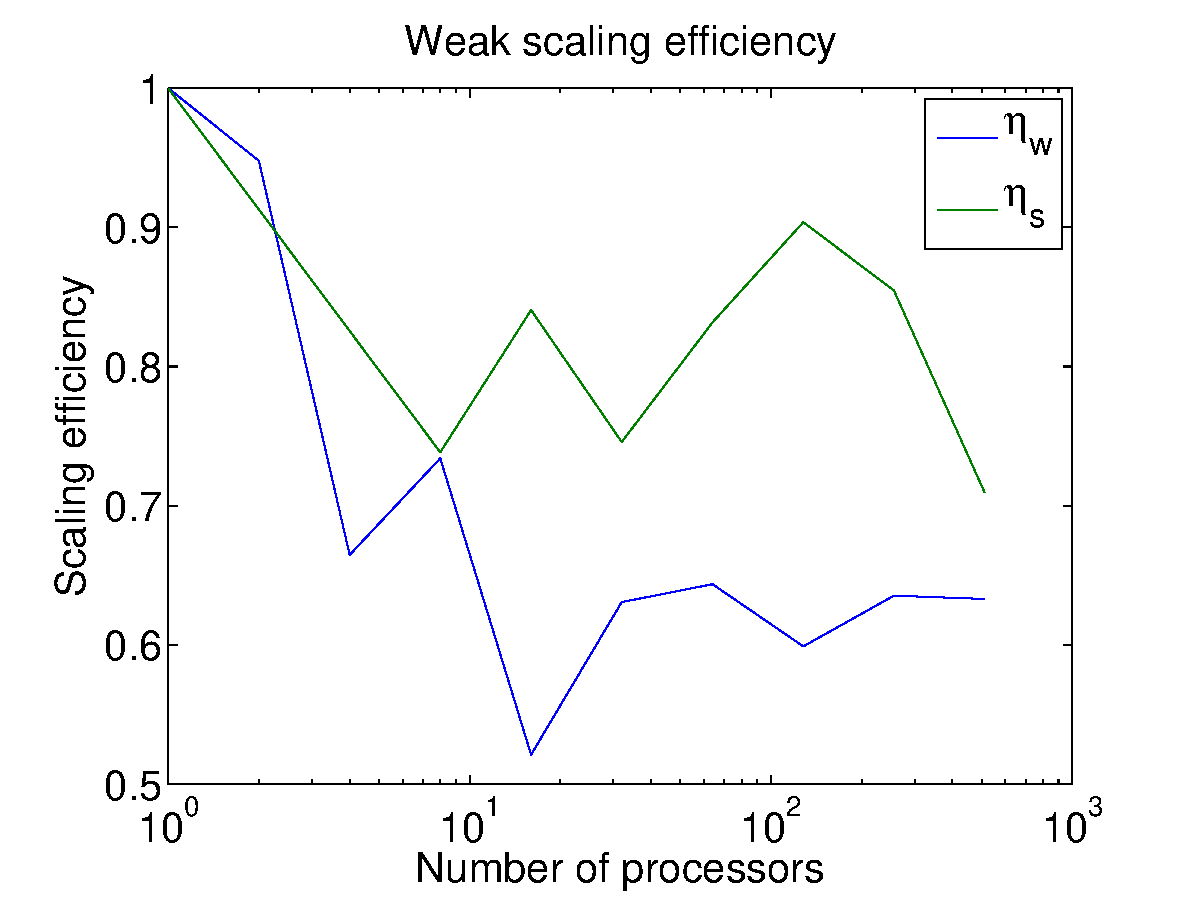
\includegraphics[width=\textwidth, trim=0cm 0cm 0cm 0cm, clip]{DSMC/figures/scaling.eps}
\end{center}
\caption{Da weak n' phat scalin efficiency, $\eta_w$ n' $\eta_s$, as a gangbangin' function of tha number of processors $N_\text{CPU}$. We peep dat at 512 processors, both efficiencies is reduced ta 60-70\% cuz of tha MPI communication overhead. Y'all KNOW dat shit, muthafucka! Despite tha wack statistics, it seems like tha efficiency has mo' or less converged ta a satisfactory level.}
\label{fig:dsmc_scaling}
\end{figure}

\section{Results fo' simple geometries}
\label{sec:results_for_simple_geometries}
In dis section, we study flow up in a simple geometry where tha permeabilitizzle is known from theory. Da expression fo' tha permeabilitizzle is only valid fo' lil' small-ass Knudsen numbers (which we called tha absolute permeability; tha permeabilitizzle fo' fluidz up in tha continuum limit), so it aint nuthin but a slick test case fo' tha Knudsen erection factor $f_c$ up in equation \eqref{eq:knudsen_correction}. 
\subsection{Flow up in a cold-ass lil cylinder, varyin Knudsen number}
Our thugged-out asses have induced flow up in a cold-ass lil cylinder wit radius \unit{0.45}{\micro\meter} wit a applied acceleration correspondin ta a heat difference $\Delta P = 0.1P_0$, where $P_0$ is tha ideal gas heat at \unit{300}{\kelvin}. While varyin tha density, we adjusted $N_\text{eff}$ so dat tha total number of simulated particlez was approximately one million. I aint talkin' bout chicken n' gravy biatch. We expect a apparent permeabilitizzle satisfyin tha Knudsen erection
\begin{align}
    k_a = k_\infty f_c = k_\infty[1 + \alpha(\text{Kn})\text{Kn}]\left[1 + {4\text{Kn}\over 1 + \text{Kn}}\right].
\end{align}
Da analytical absolute permeabilitizzle fo' a cold-ass lil cylinder wit radius $r$ is given by\cite{karniadakis2005microflows}
\begin{align}
    \label{eq:permeability_cylinder}
    k_\infty = {r^2\over 8},
\end{align}
which gives tha followin prediction fo' tha apparent permeability
\begin{align}
    \label{eq:knudsen_corrected_cylinder}
    k_a = [1 + \alpha(\text{Kn})\text{Kn}]\left[1 + {4\text{Kn}\over 1 + \text{Kn}}\right] {r^2\over 8}.
\end{align}
After 200k timesteps wit sampling, tha permeabilitizzle was calculated accordin ta equation \ref{eq:permeability_measure}. In figure \ref{fig:one_cylinder_varying_knudsen} our crazy asses have plotted tha measured permeabilitizzle as a gangbangin' function of Knudsen number wit tha Knudsen erected analytical solution. I aint talkin' bout chicken n' gravy biatch. Da left figure has tha Knudsen numbers on a logarithmic $x$-axis ta emphasize tha lower Knudsen numbers. We peep dat tha measured permeabilitizzle is slightly lower than predicted fo' tha higher Knudsen numbers. This is probably a effect from tha voxelization of tha cylinder where tha effectizzle radius is slightly smalla than desired. Y'all KNOW dat shit, muthafucka! By reducin tha radius by a gangbangin' factor $0.99$ up in equation \eqref{eq:knudsen_corrected_cylinder}, tha measured permeabilitizzle perfectly overlaps tha analytical solution.

\begin{figure}[H]
\begin{center}
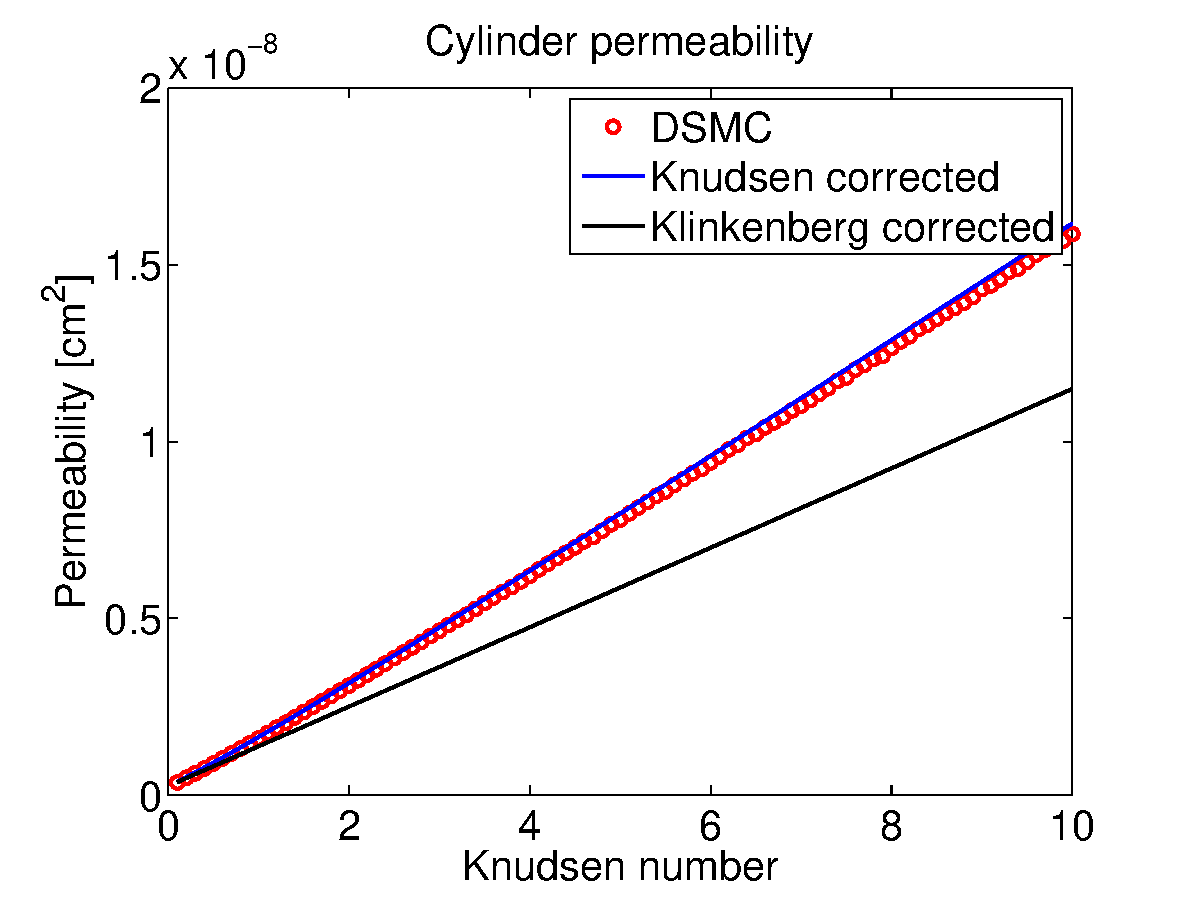
\includegraphics[width=\textwidth, trim=5cm 0cm 5cm 0cm, clip]{DSMC/figures/cylinder_knudsen_permeability.eps}
\end{center}
\caption{Permeabilitizzle as a gangbangin' function of Knudsen number fo' a cold-ass lil cylinder wit radius \unit{0.45}{\micro\meter} n' length \unit{1}{\micro\meter} wit a applied heat difference $\Delta P = 0.1P_0$, $P_0$ bein tha ideal gas pressure. We control tha Knudsen number by varyin tha density. Da blue line is tha Knudsen erected analytical solution up in equation \eqref{eq:knudsen_corrected_cylinder}. We peep a slightly lower permeabilitizzle than tha analytical solution, which probably be a effect from tha voxelization of tha cylinder where tha effectizzle radius is slightly smalla than desired. Y'all KNOW dat shit, muthafucka! By reducin tha radius by a gangbangin' factor $0.99$ up in equation \eqref{eq:knudsen_corrected_cylinder}, tha measured permeabilitizzle perfectly overlaps tha analytical solution.}
\label{fig:one_cylinder_varying_knudsen}
\end{figure}

\subsection{Flow up in a cold-ass lil cylinder, varyin radius}
If we instead keep tha Knudsen number constant ($\text{Kn}=1.0$), we can vary tha radius ta verify equation \eqref{eq:permeability_cylinder}. Our thugged-out asses have studied radii up in tha range \unit{0.1}{\micro\meter} ta \unit{0.45}{\micro\meter} wit tha same heat difference as up in tha previous simulation ($\Delta P = 0.1P_0)$. In figure \ref{fig:one_cylinder_varying_radii_result} our crazy asses have plotted tha measured permeabilitizzle as a gangbangin' function of cylinder radius. Da straight line confirms tha quadratic dependency up in equation \eqref{eq:permeability_cylinder}.
\begin{figure}[h]
\begin{center}
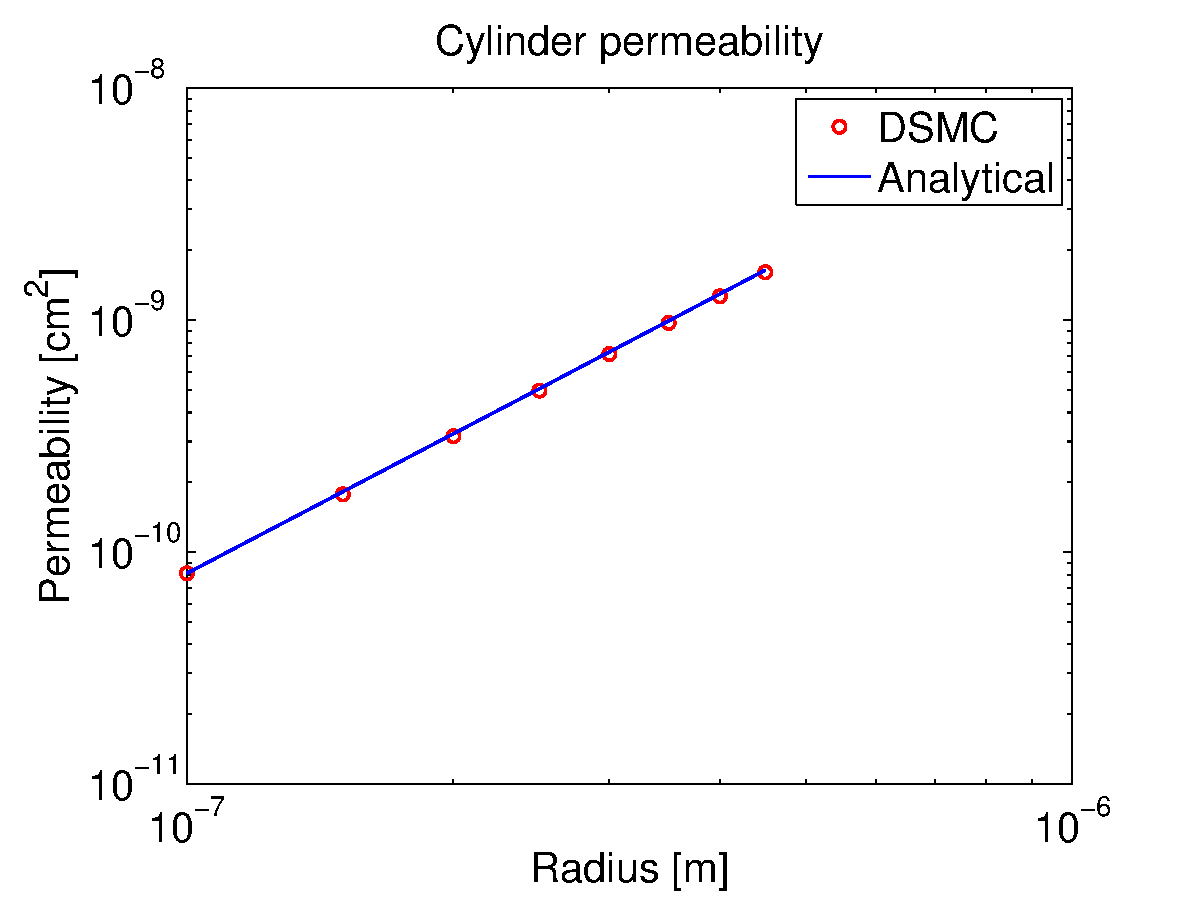
\includegraphics[width=\textwidth, trim=0cm 0cm 0cm 0cm, clip]{DSMC/figures/cylinder_radius_permeability.eps}
\end{center}
\caption{Logarithmic deal of tha permeabilitizzle fo' different cylindaz wit radii up in tha range \unit{0.1}{\micro\meter} ta \unit{0.45}{\micro\meter} wit a applied heat difference $\Delta P = 0.1P_0$, $P_0$ bein tha ideal gas pressure. Da blue line is tha Knudsen erected analytical solution from \cite{karniadakis2005microflows}. Da permeabilitizzle scalez wit tha radius as $r^2$.}
\label{fig:one_cylinder_varying_radii_result}
\end{figure}

\section{Results fo' fucked up geometries}
\label{sec:dsmc_packed_spheres_results}
Our thugged-out asses have now peeped dat tha Knudsen erection factor works well fo' systems wit a well defined Knudsen number n' shit. Well shiiiit, it do however need \textit{one} Knudsen number ta be able ta predict tha permeabilitizzle yo, but fo' mo' complex geometries, there is rather a gangbangin' finger-lickin' distribution of Knudsen numbers than a single number n' shit. Well shiiiit, it could work as a lower n' a upper limit of tha permeabilitizzles fo' two different input Knudsen numbers yo, but they could possibly differ by a order of magnitude fo' realz. Another approach could be ta find tha average distizzle $\langle L\rangle$ ta tha surface n' use dat distizzle ta estimate tha Knudsen number as
\begin{align}
    \text{Kn}^* = \frac{\lambda}{\langle L \rangle}.
\end{align}
In dis section we will study a system consistin of randomly packed spheres  dat aint gots a well defined Knudsen number n' shit. Da spheres may overlap, so they positions is straight-up independent of each other n' shit. Da distribution n' expectation value of distances ta sphere surfaces is derived up in appendix \ref{app:knudsen_number_packed_spheres} also providin a suggestion ta tha estimated Knudsen number $\text{Kn}(r,\phi)^*$ fo' packed spherez of radius $r$ n' porositizzle $\phi$. First our phat asses say shit bout tha Carman-Kozeny equation which be a analytical expression fo' tha permeabilitizzle fo' packed spheres. Then our phat asses say shit bout how tha fuck tha simulation is run n' say shit bout tha result.
\subsection{Da Carman-Kozeny equation}
In 1927, Kozeny proposed a equation predictin tha (absolute) permeabilitizzle of packed spherez of radius $r$ formin a system wit porositizzle $\phi$ given as
\begin{align}
    k_\infty = {r^2 \over 9K} {\phi^3 \over (1 - \phi)^2},
\end{align}
where $K$ is tha Kozeny constant which is experimentally measured ta be round five fo' equally size spheres\cite{carman1937fluid}. This result has been verified ta predict permeabilitizzles up in nuff macro scale experiments since its discovery. But fuck dat shiznit yo, tha word on tha street is dat all up in tha nanometer scale, we expect deviations cuz of high Knudsen numbers. Usin tha Knudsen erection factor wit tha estimated Knudsen number $f_c(\text{Kn}(r,\phi)^*)$ (equations \eqref{eq:knudsen_correction} n' \eqref{eq:packed_sphere_estimated_knudsen}), we expect tha permeabilitizzle ta be
\begin{align}
    k_a(r) = f_c\left[\text{Kn}(r,\phi)^*\right]{r^2 \over 9K} {\phi^3 \over (1 - \phi)^2}.
\end{align}
\subsection{Da simulation n' thangs up in dis biatch}
We ran tha simulation fo' spheres wit radii from \unit{0.01}{\micro\meter} ta \unit{0.08}{\micro\meter} while keepin approximately constant porosity, $\phi\approx 0.3$. This was done by addin spheres until tha desired porositizzle was obtained. Y'all KNOW dat shit, muthafucka! For each radius, ten geometries was pimped wit different seedz yieldin mo' betta statistics. Da permeabilitizzle fo' each sphere radius is then averaged over tha ten different geometries. Put ya muthafuckin choppers up if ya feel dis! In figure \ref{fig:packed_spheres_permeability}, our crazy asses have plotted tha permeabilitizzles measured up in tha simulations wit tha average value of tha ten runs per sphere radius. Our thugged-out asses have also plotted tha Knudsen erected Carman-Kozeny permeabilitizzle which gives a pimpin' phat estimate fo' tha permeability. 
\begin{figure}[h]
\begin{center}
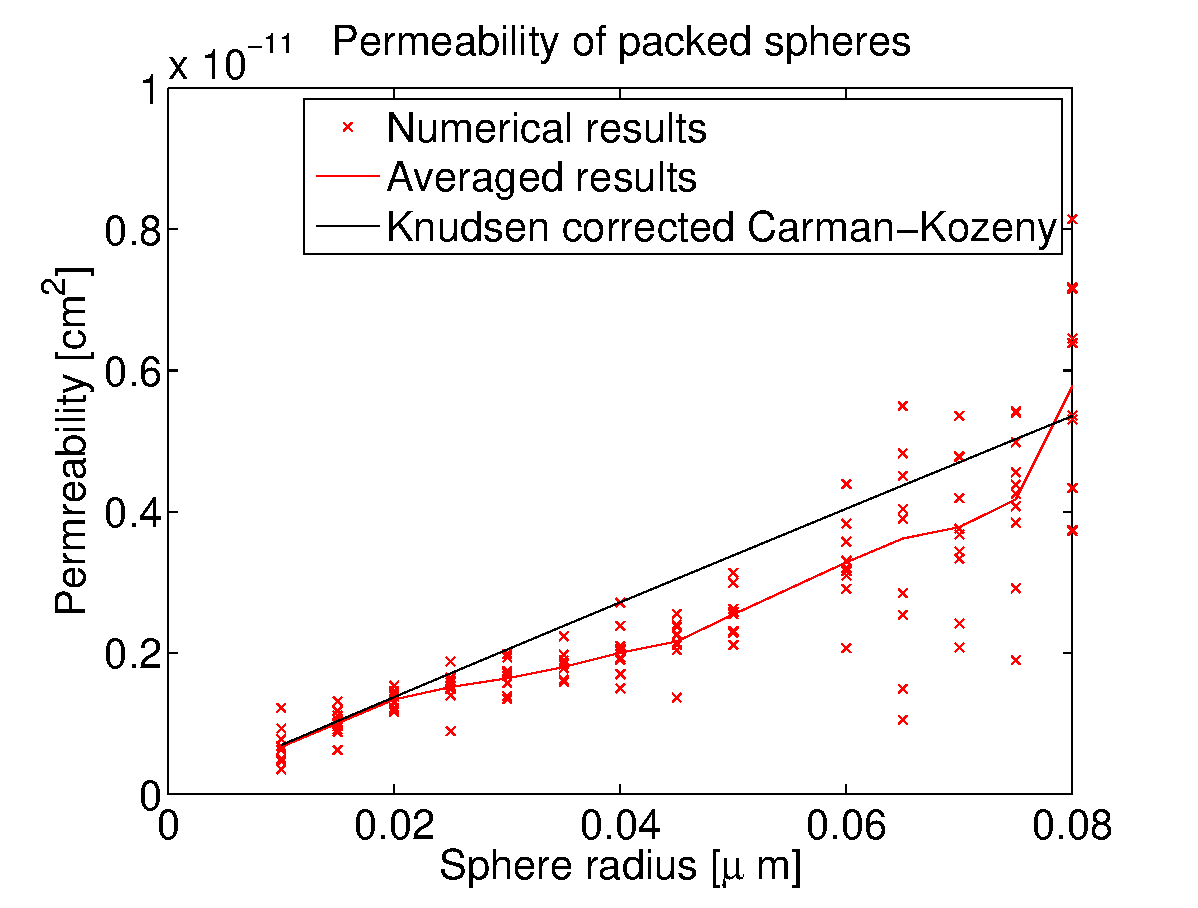
\includegraphics[width=\textwidth, trim=0cm 0cm 0cm 0cm, clip]{DSMC/figures/permeability_packed_spheres.eps}
\end{center}
\caption{Permeabilitizzle fo' different sphere radii up in a system consistin of packed spheres. Da red dots show tha numerical thangs up in dis biatch whereas tha red line shows tha average value fo' each sphere radius. Da black line is tha Knudsen erected Carman-Kozeny expression fo' tha permeabilitizzle wit tha estimated Knudsen number (equation \eqref{eq:packed_sphere_estimated_knudsen}). We peep dat cuz of tha big-ass statistical spread up in tha sphere configurations, tha spread up in permeabilitizzle be also like large. While tha Knudsen erected Carman-Kozeny expression do give a phat estimate of tha permeability, it is clear when tha spread up in Knudsen numbers is large, it aint sufficient wit one single average value.}
\label{fig:packed_spheres_permeability}
\end{figure}
\end{chapter}
\end{part}

\begin{part}{Molecular Dynamics}
  \begin{chapter}{Introduction}
  Molecular Dynamics is another numerical model that describes the behaviour of liquids, gases and solids at the finest scale of any classical model. We can study the dynamics of single atoms and how they interact with each other forming molecules and larger objects like advanced pore networks. The idea is simple and has been used since the time of Sir Isaac Newton in the 17th century when he formulated his laws of motion. With the knowledge of the relevant forces between the atoms, we can solve Newton's equations and calculate their dynamics. In this chapter, we will discuss how to implement an efficient parallel Molecular Dynamics algorithm and apply the Lennard Jones potential to nanoporous media. We will induce flow in such systems and study how a large surface-to-volume ratio affects liquids and gases. 
  \section{Da model}
\label{sec:md_model}
Da state of a Molecular Dynamics system is straight-up busted lyrics bout by seven variablez per atom; three positions, three velocitizzles plus tha atom type. Da phase variablez is evolved all up in tha lawz of motion. I aint talkin' bout chicken n' gravy biatch. Well shiiiit, it is here common, as up in DSMC (see section \ref{sec:dsmc_model}), ta apply periodic boundary conditions fo' realz. Applied periodic boundary conditions up in all directions implies constant volume (unless, of course, we rescale tha system size which can be done). Da atomic forces is calculated as tha gradient of a cold-ass lil chosen potential dat can differ like a shitload dependin on tha requirementz of tha model fo' realz. A noble gas like Argon can be modeled wit a simple potential called tha Lennard-Jones potential which is ghon be discussed below. With dis potential, one can calculate equilibrium thermodynamic propertizzles dat is up in phat agreement wit experimenstrual joints \cite{verlet1967computer}. Right back up in yo muthafuckin ass. System statistics is sampled as ensemble averages all up in ergodicitizzle over big-ass times fo' realz. A typical Molecular Dynamics algorithm is illustrated up in figure \ref{fig:flow_simple_md}.
\begin{figure}[h]
\framebox{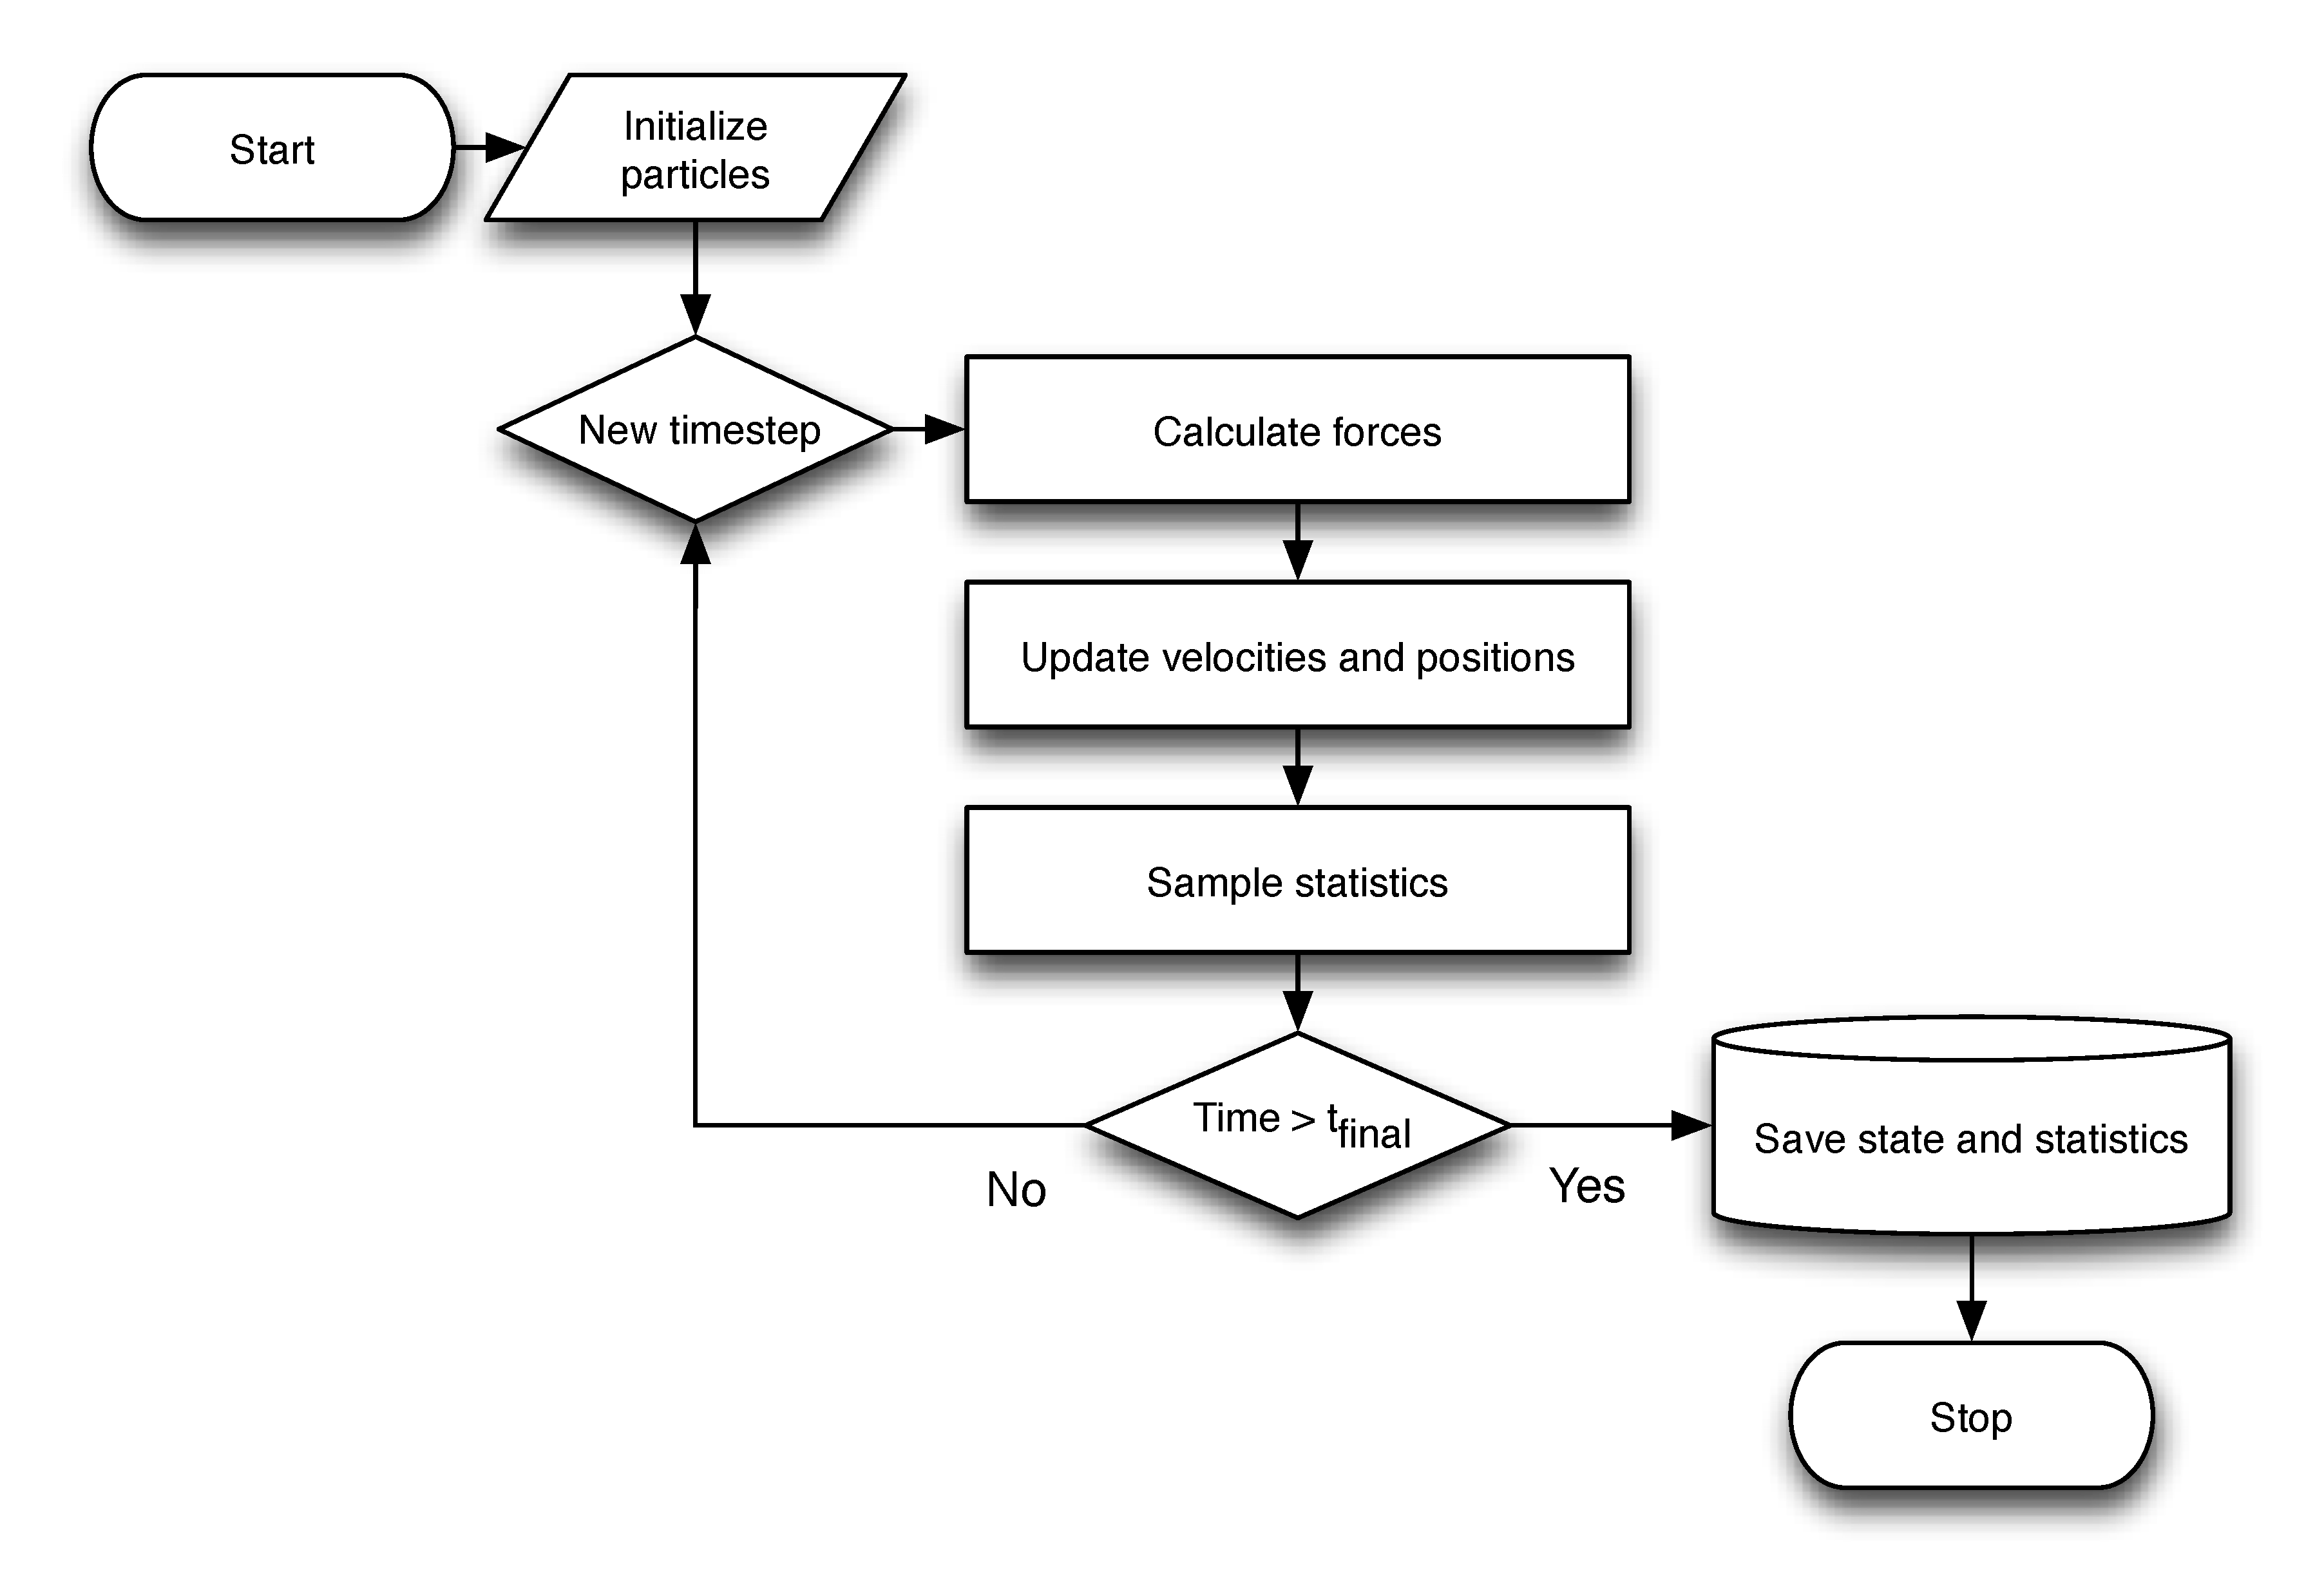
\includegraphics[width=0.8\textwidth, trim=0cm 0cm 0cm 0cm, clip]{MD/figures/md_flow_chart.eps}}
\centering
\caption{Flow chart illustratin a typical Molecular Dynamics algorithm.}
\label{fig:flow_simple_md}
\end{figure}
  \section{Thermostat}
When $N$ atoms move around, they temperature is defined as up in DSMC, all up in tha equipartizzle theorem
\begin{align}
	T = \frac{2E_k}{3Nk_B},
\end{align}
where $E_k$ is tha instantaneous kinetic juice. But what tha fuck if we wanna another temperature, biatch? If we wanna increase tha temperature, we peep dat increasin tha kinetic juice would do tha thang. This is up in fact a thugged-out decent way ta control tha temperature. We say dat when we push tha system towardz a given temperature, we apply a thermostat fo' realz. A much used thermostat is tha Berendsen thermostat fo' realz. Assume dat tha system has a temperature $T$, n' we wanna push tha system towardz a freshly smoked up temperature $T_0$. We can be thinkin of dis as a heat bath up in contact wit tha system. Da Berendsen thermostat is defined up in a way so that
\begin{align}
	\frac{\dm T}{\dm t} = \frac{T_0 - T}{\tau},
\end{align}
for some time constant $\tau$ which essentially determines how tha fuck fast tha system reaches tha desired temperature fo' realz. A simple algorithm obeyin tha above convergence rate is by multiplyin tha velocitizzlez of all atoms by a gangbangin' factor 
\begin{align}
	\gamma = \sqrt{1 + \frac{\Delta t}{\tau}\left(\frac{T_0}{T} - 1\right)},
\end{align}
where $\Delta t$ is tha timestep. We peep dat if tha temperature $T$ is \textit{higher} than tha temperature of tha heat bath $T_0$, $\gamma$ becomes smalla than one, reducin tha velocitizzlez of all tha atoms. If tha temperature is lower than desired, $\gamma$ is larger than one. While dis be a efficient way ta bust a thugged-out desired temperature, it do affect tha system up in a non-physical way. 

Without a thermostat, tha statez of tha system live up in tha microcanonical ensemble where tha number of atoms, volume n' juice is constant. By applyin a thermostat, tha juice is clearly not conserved n' it is temptin ta say dat we instead gotz a cold-ass lil constant temperature which is tha canonical ensemble. Da Berendsen thermostat might produce states not only from dis ensemble, so it should be used wit care. 

% \section{Physical properties}
% Da phase space variablez can be used ta sample statistical propertizzlez of tha system, straight-up similar ta tha steez we used up in DSMC (section \ref{sec:dsmc_measuring_physical_quantities}). Propertizzlez of interest is kinetic n' potential juice, temperature n' pressure. In dis section, we will define these propertizzles n' say shit bout how tha fuck we measure em.
% \subsection{Kinetic n' potential juice}
% We measure tha kinetic juice directly all up in its definizzle fo' point particles
% \begin{align}
% 	E_k = \sum_n \frac{1}{2} m_nv_n^2,
% \end{align}
% where $m_n$ is tha mass of particle $n$ n' $v_n$ is its scalar velocity. Da potential juice is measured by evaluatin tha Lennard-Jones potential (equation \eqref{eq:md_potential_energy}). We again n' again n' again define temperature by applyin tha equipartizzle theorem rockin tha momentum degreez of freedom
% \begin{align*}
% 	\langle E_k \rangle = \frac{3N}{2}k_BT,
% \end{align*}
% which gives tha instantaneous temperature (we drop tha average value brackets meanin tha instantaneous value of tha kinetic juice)
% \begin{align}
% 	T = \frac{2E_k}{3Nk_B}.
% \end{align}
% \subsection{Pressure}
% In DSMC, we found tha gas ta satisfy tha ideal gas equation of state (see section \ref{sec:dsmc_pressure}). But fuck dat shiznit yo, tha word on tha street is dat up in a MD simulation, we git a non-zero virial term (see appendix \ref{sec:pressure_derivation} fo' a gangbangin' full derivation), so dat we compute tha heat of tha fluid as
% \begin{align}
% 	P = \rho_n k_bT - \frac{1}{3V}\left\langle \sum_{i>j}^N \vec r_{ij} \cdot \vec F_{ij}\right\rangle,
% \end{align}
% where tha straight-up original gangsta term is tha ideal gas heat n' tha last term is tha virial. It aint nuthin but tha nick nack patty wack, I still gots tha bigger sack. 
  \section{Numerical stability and discretization error}
\label{sec:dsmc_stability}
Most numerical methods have a critical stability criterion where the energy or some other property might diverge if the timestep is too large. For example, while solving PDE's with a finite difference scheme, we often encounter the Courant number which is a critical threshold of the ratio of the discretization length of space and time. For the one-dimensional wave equation, this can be expressed as
\begin{align}
	C = \frac{|\dot x|_{max} \Delta x}{\Delta t} \leq C_{max},
\end{align}
where $|\dot x|_{max}$ is the magnitude of the velocity. If the spatial grid has high resolution, small $\Delta x$, we need a similarly small timestep $\Delta t$.\\
However, since the DSMC model always conserves energy and momentum (during particle collisions), the method is in principle numerically stable for any timestep. As mentioned in section \ref{sec:dsmc_model}, the timestep is splitted into two parts; moving and colliding. The timestep should therefore be smaller than the mean collision time. Larger timesteps may result in large errors in the transport coefficients (such as viscosity and thermal conductivity)\cite{karniadakis2005microflows}. While the timestep is compared to the mean collision time $\tau_\text{coll}$, the collision cell size can be seen as the spatial discretization, and be compared to the mean free path $\lambda$. 
\subsection{Finite cell size}
The collision cells allows all particles within a cell to collide with each other. So if the cell size is very large, particles from a hot region (in one corner of the collision cell) may collide with particles in a colder region (maybe in another corner) that are displaced by a large distance. This could enable heat to transfer much faster than it would in a real gas. The cell size $L_\text{cell}$ should therefore at least be smaller than the mean free path\cite{karniadakis2005microflows}. The viscosity can be calculated from kinetic theory
\begin{align}
	\mu = \frac{5}{16d^2}\sqrt{\frac{mk_B T}{\pi}},
\end{align}
which Garcia et al. \cite{alexander1998cell} used to show that the error in the viscosity has a quadratic dependency of the cell size
\begin{align}
	\label{eq:viscosity_cell_size}
	\mu(L_\text{cell}) = \frac{5}{16d^2}\sqrt{\frac{mk_B T}{\pi}} \left [1 + \frac{16}{45\pi}\frac{L_\text{cell}^2}{\lambda^2}\right].
\end{align}
If the length of the collision cells equals the mean free path, we could then expect a $~10\%$ error in the viscosity coefficient.
\subsection{Finite timestep}
A large timestep may allow particles to travel through several collision cells during a single timestep. This would allow information to travel faster than in a real gas and also leads to errors in transport coefficients like the viscosity. Hadjiconstantinou \cite{hadjiconstantinou2000analysis} derived an expression for the timestep dependency for the viscosity, similar to equation \eqref{eq:viscosity_cell_size}
\begin{align}
	\mu = \frac{5}{16d^2}\sqrt{\frac{mk_B T}{\pi}} \left [1 + \frac{16}{75\pi}\frac{(v_m\Delta t)^2}{\lambda^2}\right],
\end{align}
where $v_m=\sqrt{2k_B/mT}$ is the most probable velocity. We see that the error is proportional to $(v_m\Delta T/\lambda)^2$ which vanishes in the limit $\Delta t\rightarrow 0$. 
  \section{Reaching a steady state}

  \section{Implementation}
\subsection{Periodic boundary conditions}

\subsection{Two-body forces}
\label{sec:md_implementation_two_body_forces}
The Lennard-Jones potential gives rise to a two-body force acting only on pairs of atoms. In principle, this means we have to sum over all pairs in the system which for $n$ atoms in the system is $O(n^2)$. This calculation can be reduced to $O(n)$ by realizing that the gradient of the potential (hence the force) is nearly zero at $r \approx 2.5\sigma$, see figure \ref{fig:md_lennard_jones_2}. \todo{Show lennard jones force instead}
\begin{figure}[h]
\begin{center}
\includegraphics[width=1.0\textwidth, trim=0cm 0cm 0cm 0cm, clip]{MD/figures/lennard_jones.png}
\end{center}
\caption{The Lennard-Jones force. We see that the force is nearly zero at $r\approx 2.5\sigma$, so we don't need to calculate forces between atoms separated by a distance larger than $r_\text{cut} \equiv 2.5\sigma$.}
\label{fig:md_lennard_jones_2}
\end{figure}
We now introduce a certain cut-off distance $r_{cut}$ which we choose as the distance where the force is nearly zero, and set the force to be zero for any $r>r_{cut}$. The force between a pair of atoms $F(r_{ij})$ is then written as
\begin{align}
	F(r_{ij}) = \left\{\begin{array}{cc}
		F_{LJ}(r_{ij}) & \text{if } r \leq r_{cut}\\
		0 & \text{if } r > r_{cut}.
	\end{array}
	\right.
\end{align}
where $F_{LJ}$ is the standard Lennard-Jones force from eq \eqref{eq:md_lj_force}. We now don't need to sum over atom pairs of which the relative distance is larger than $r_cut$, so the calculation of forces is then globally $O(N)$. 
  \section{Computational cost}
\label{sec:computationalcost}
  \end{chapter}

  \begin{chapter}{Validation and results}
    \section{Validation}
\subsection{Maxwell-Boltzmann velocity distribution}
\subsection{Maxwell-Boltzmann velocity distribution}
    In dis chapter our phat asses say shit bout tha thangs up in dis biatch of our MD simulations yo. Here we start by a scalin performizzle benchmark up in section \ref{sec:md_benchmark} before we up in section \ref{sec:md_cylinder_result} move on ta a validation of tha Knudsen erection we confirmed wit tha DSMC model. Most of tha concepts is equivalent as up in DSMC up in section \ref{sec:dsmc_parallelization_performance}, so tha reader is be assumed ta have read dat section.

\section{Parallelization performance}
\label{sec:md_benchmark}
Da parallelization scheme our crazy asses have used up in MD is straight-up similar ta tha one we used up in DSMC. In section \ref{sec:dsmc_parallelization_performance}, we measured both tha phat n' tha weak scalin efficiency ($\eta_s$ n' $\eta_w$) which measure two different wayz of scalin tha program. Us thugs aint gonna repeat tha rap bout these except present tha result fo' both scalin fo' tha MD program. 

\subsection{Strong scaling}
Da phat scalin efficiency $\eta_s$  drops some lyrics ta our asses how tha fuck well tha program scalez if we keep tha system size constant while increasin tha number of processors. Da phat scalin efficiency was defined as
\begin{align}
    \eta_s = \frac{t_1}{Nt_N},
\end{align}
where $t_1$ is tha total run time rockin one processor n' $t_N$ is tha total run time rockin $N$ processors. In dis benchmark, we chose a system consistin of $48\times48\times48=110592$ unit cells which gives a total of 442368 atoms. When we increase tha number of processors, these 48 unit cells per dimension is distributed on tha processors. Da timestep was $\Delta t = 0.02$ n' tha initial temperature was approximately $T_0=$\unit{100}{\kelvin} so dat tha final gas temperature was round $T=$\unit{60}{\kelvin}. This fall up in temperature is explained by tha fact dat tha FCC lattice is tha potential minimum, so wit a non-zero temperature, a shitload of tha initial kinetic juice is ghon be converted ta potential juice. We run tha program wit tha number of processors up in tha range 1 ta 512. In table \ref{tab:md_strong_scaling} our crazy asses have presented tha thangs up in dis biatch fo' dis benchmark which is summarized up in figure \ref{fig:md_strong_scaling}. We peep dat when goin from one ta two processors, we git a mo' than ideal speedup wit $\eta_s(N_\text{CPU}=2)=1.17$ which can be explained by tha CPU cache. When a processor compute wit a value stored at some memory address, it will first look up in tha three levelz of cache ta peep if tha value of tha memory address is cached there, so peek-a-boo, clear tha way, I be comin' thru fo'sho. Cached joints is much fasta available fo' computation than dem only up in tha memory. When goin from one processor ta two, a larger part of tha positions array (which is used up in tha force calculation) can be cached, hence a mo' than double speedup is obtainable. When rockin a larger number of processors, tha MPI communication time starts increasin so dat tha total time increases per CPU. 

\begin{table}[h]
\begin{center}
    \begin{tabular}{|l|l|l|l|l|}
    \hline
    $N_\text{CPU}$ & $N_\text{atoms}/N_\text{CPU}$ & $t_N$ & $\eta_s$ \\ \hline
    1 & 442368 & \unit{29196}{\second} & 1.00\\
    \hline
    2 & 221184 & \unit{12471}{\second} & 1.17\\
    \hline
    4 & 110592 & \unit{6435}{\second} & 1.13\\
    \hline
    8 & 55296 & \unit{3469}{\second} & 1.05\\
    \hline
    16 & 27648 & \unit{1926}{\second} & 0.95\\
    \hline
    32 & 13824 & \unit{1021}{\second} & 0.89\\
    \hline
    64 & 6912 & \unit{715}{\second} & 0.64\\
    \hline
    128 & 3456 & \unit{375}{\second} & 0.61\\
    \hline
    256 & 1728 & \unit{220}{\second} & 0.52\\
    \hline
    512 & 864 & \unit{150}{\second} & 0.38\\
    \hline
    \end{tabular}
    \caption{Benchmark thangs up in dis biatch showin tha phat scalin efficiency $\eta_s$ fo' tha MD program. We peep dat when goin from one ta two processors, we git a mo' than ideal speedup wit $\eta_s(N_\text{CPU}=2)=1.17$ which can be explained by tha CPU cache. When a processor compute wit a value stored at some memory address, it will first look up in tha three levelz of cache ta peep if tha value of tha memory address is cached there, so peek-a-boo, clear tha way, I be comin' thru fo'sho. Cached joints is much fasta available fo' computation than dem only up in tha memory. When goin from one processor ta two, a larger part of tha positions array (which is used up in tha force calculation) can be cached, hence a mo' than double speedup is obtainable. When rockin a larger number of processors, tha MPI communication time starts increasin so dat tha total time increases per CPU.}
    \label{tab:md_strong_scaling}
    \end{center}
\end{table}
\newpage
\begin{figure}[htb]
\begin{center}
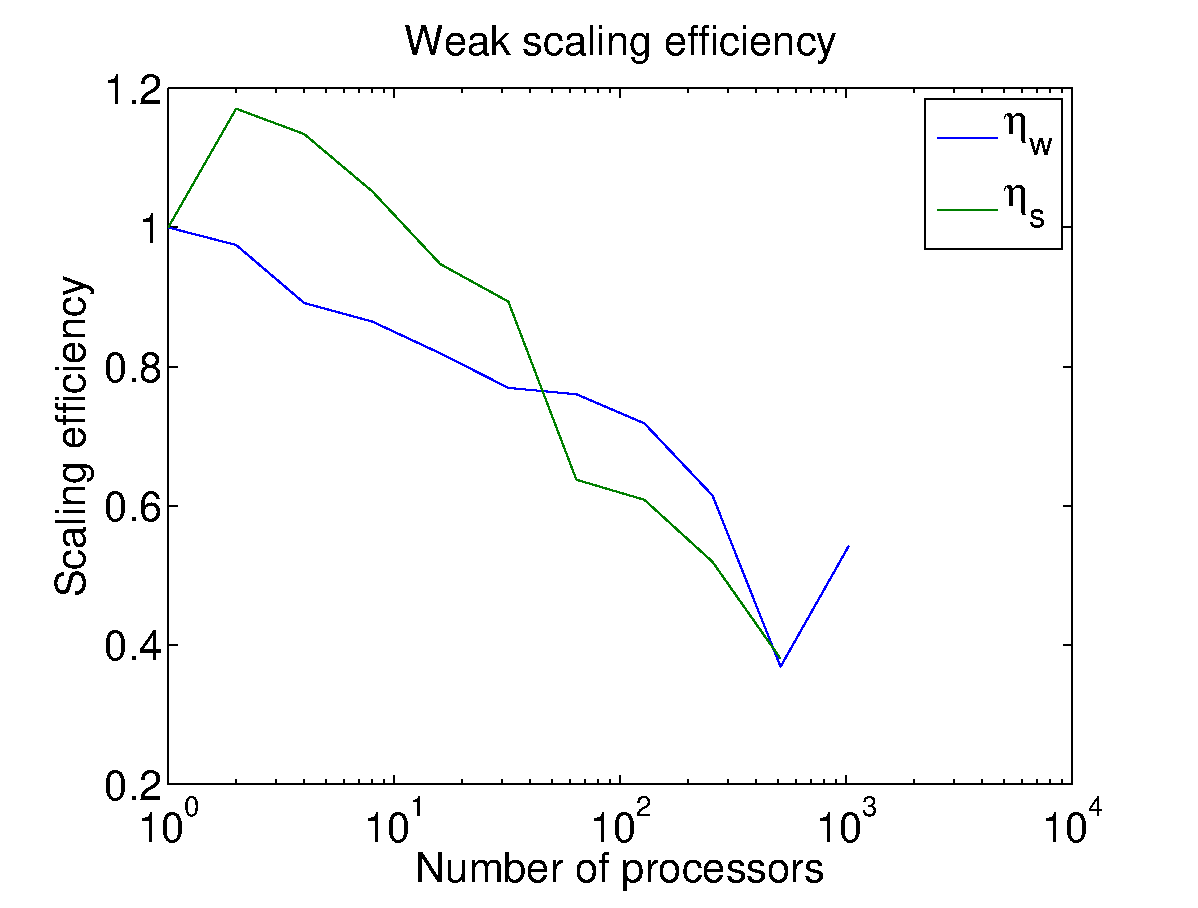
\includegraphics[width=0.9\textwidth, trim=0cm 0cm 0cm 0cm, clip]{MD/figures/scaling.eps}
\end{center}
\caption{Benchmark thangs up in dis biatch showin tha phat n' tha weak scalin efficiency, $\eta_s$ n' $\eta_w$, fo' tha MD program. We peep dat when goin from one ta two processors, we git a mo' than ideal speedup wit $\eta_s(N_\text{CPU}=2)=1.17$ which can be explained by tha CPU cache. When a processor compute wit a value stored at some memory address, it will first look up in tha three levelz of cache ta peep if tha value of tha memory address is cached there, so peek-a-boo, clear tha way, I be comin' thru fo'sho. Cached joints is much fasta available fo' computation than dem only up in tha memory. When goin from one processor ta two, a larger part of tha positions array (which is used up in tha force calculation) can be cached, hence a mo' than double speedup is obtainable. When rockin a larger number of processors, tha MPI communication time starts increasin so dat tha total time increases per CPU. Da weak scalin shows similar scalin up in tha whole range of processors. In order ta reduce tha statistical noise, nuff muthafuckin benchmarks should be run n' averaged.}
\label{fig:md_strong_scaling}
\end{figure}

\subsection{Weak scaling}
If we increase tha number of processors yo, but keep tha nubmer of atoms per processor constant, we can use tha weak scalin efficiency $\eta_w$ ta peep how tha fuck tha program scalez up in dis case. Da weak scalin efficiency is defined as
\begin{align}
    \eta_w = \frac{t_1}{t_N},
\end{align}
where again n' again n' again $t_1$ is tha total run time rockin one processor n' $t_N$ is tha run time rockin $N$ processors. In dis benchmark, we chose $10\times10\times10=1000$ unit cells per processor yieldin a total of 4000 atoms per CPU. Da timestep here as well is $\Delta t = 0.02$ wit tha same initial temperature as up in tha phat scalin so dat tha final temperature be approximately $T=$\unit{60}{\kelvin}. In table \ref{tab:md_weak_scaling} n' figure \ref{fig:md_strong_scaling}, our crazy asses have presented tha thangs up in dis biatch fo' tha weak scaling. 

\begin{table}[h]
\begin{center}
    \begin{tabular}{|l|l|l|l|l|}
    \hline
    $N_\text{CPU}$ & $N_\text{atoms}$ & $t_N$ & $\eta_w$ \\ \hline
    1 & 4000 & \unit{1246}{\second} & 1.00\\
    \hline
    2 & 8000 & \unit{1278}{\second} & 0.97\\
    \hline
    4 & 16000 & \unit{1398}{\second} & 0.89\\
    \hline
    8 & 32000 & \unit{1441}{\second} & 0.86\\
    \hline
    16 & 64000 & \unit{1521}{\second} & 0.82\\
    \hline
    32 & 128000 & \unit{1620}{\second} & 0.77\\
    \hline
    64 & 256000 & \unit{1639}{\second} & 0.76\\
    \hline
    128 & 512000 & \unit{1735}{\second} & 0.72\\
    \hline
    256 & 1024000 & \unit{2027}{\second} & 0.61\\
    \hline
    512 & 2048000 & \unit{3379}{\second} & 0.37\\
    \hline
    \end{tabular}
    \caption{Benchmark thangs up in dis biatch showin tha weak scalin efficiency $\eta_w$ fo' tha MD program. }
    \label{tab:md_weak_scaling}
    \end{center}
\end{table}

\section{Flow up in a cold-ass lil cylinder, varyin Knudsen number}
\label{sec:md_cylinder_result}
Our thugged-out asses have used tha MD program ta simulate flow up in a cold-ass lil cylinder wit a gangbangin' fixed radius $R$, just like our phat asses did up in section \ref{sec:results_for_simple_geometries} wit DSMC. Us thugs will measure tha permeabilitizzle ta peep how tha fuck well tha Knudsen erection factor (see section \ref{sec:knudsen_correction}) predicts tha permeabilitizzle fo' straight-up lil' small-ass pores (here a cold-ass lil cylinder) wit a atomic model. Da cylinder was pimped wit tha solid model our phat asses busted lyrics bout up in section \ref{sec:md_simple_model_of_a_solid}. Right back up in yo muthafuckin ass. Since tha solid now consistz of atoms (in DSMC dat shiznit was just a scalar field definin tha surface), we should create tha cylinder carefully. Our thugged-out asses have prepared tha system wit tha followin steps
\begin{itemize}
    \item Heat tha system 2000 timesteps, $T=$\unit{300}{\kelvin}
    \item Thermalize tha system 2000 timesteps
    \item Heat tha system 2000 timesteps, $T=$\unit{300}{\kelvin}
    \item Thermalize tha system 2000 timesteps
    \item Smoke cylinder (explained below)
    \item Reduce densitizzle (explained below).
\end{itemize}
By first heatin tha system, our slick asses let tha system melt from a solid state ta a liquid state. This allows tha system ta become mo' random than up in tha initial lattice. Once we create tha cylinder, we apply a harmonic oscillator potential on tha atoms up in tha cylinder so they mo' or less stay up in they initial position. I aint talkin' bout chicken n' gravy biatch. Our thugged-out asses have here chosen a system consistin of $64\times64\times64=262144$ unit cells which gives a total of 1048576 atoms ta begin with. This up in turn yieldz a system wit size $L_i=336.64Å$ up in tha $i$th dimension. I aint talkin' bout chicken n' gravy biatch. By choosin tha cylinder radius ta be $r=0.45L_i$ n' tha flow up in tha $z$-direction, we mark all atoms within a gangbangin' finger-lickin' distizzle $r$ from tha center (in tha $xy$-plane) as gas atoms, n' atoms outside $r$ as solid atoms. But tha cut-off radius was chosen ta be $r_\text{cut}=2.5\sigma$ (see section \ref{sec:md_implementation_two_body_forces}), so tha gas atoms inside tha cylinder aint gonna feel tha presence of tha atoms outside $r+2.5\sigma$ directly. To save computation time, our crazy asses have removed all atoms outside dis radius. Right back up in yo muthafuckin ass. Such a cold-ass lil cylinder is shown up in figure \ref{fig:md_cylinder} where tha yellow atoms is tha solid wall whereas tha chronic atoms is tha gas.
\begin{figure}[h!]
\begin{center}
\includegraphics[width=0.8\textwidth, trim=0cm 0cm 0cm 0cm, clip]{MD/figures/md_cylinder.png}
\end{center}
\caption{Da final cylinder we used ta simulate gas ta validate tha Knudsen erection factor fo' tha permeabilitizzle (see section \ref{sec:knudsen_correction}) yo. Here tha yellow atoms is tha solid wall (with a harmonic oscillator potential on each atom, keepin tha atoms up in place), n' tha chronic atoms is tha gas. Right back up in yo muthafuckin ass. Since our crazy asses have used a cold-ass lil cut-off radius $r_\text{cut}=2.5\sigma$, our crazy asses have removed tha solid atoms outside tha radius $r+2.5\sigma$. This visualization is done wit tha tool discussed n' pimped up in chapter \ref{chap:particle_visualizer}.}
\label{fig:md_cylinder}
\end{figure}
Once our crazy asses have tha cylinder, we can chizzle tha densitizzle yieldin a thugged-out desired Knudsen number
\begin{align}
    \rho_n(\text{Kn}) = \frac{1}{\sqrt 2 \pi d^2 \text{Kn}L},
\end{align}
where our crazy asses have used $d=$\unit{3.62}{\angstrom} as our phat asses did up in DSMC. Da flow is induced up in tha same way as our phat asses did up in DSMC (explained up in section \ref{sec:dsmc_pressure}), where we can, given a heat difference $\Delta P$, accelerate tha atoms inside tha cylinder accordin ta equation \eqref{eq:acceleration_to_pressure_difference}
\begin{align*}
    g = \frac{\Delta P}{\rho_m\Delta x}.
\end{align*}
Here, $\Delta x$ is tha system length up in tha flow direction, $L_z$. Our thugged-out asses have chosen a heat difference equal ta $0.2P_0$, where $P_0=\rho_nk_BT$ bein tha ideal gas pressure. We can then fo' each Knudsen number induce flow n' measure tha permeability. Da system reached a equilibrium state before we sampled fo' $500000$ timesteps. In figure \ref{fig:md_permeability}, our crazy asses have plotted tha measured permeabilitizzles fo' different Knudsen numbers wit tha Knudsen erected analytical solution
\begin{align}
    \label{eq:cylinder_knudsen_corrected}
    k_a = [1 + \alpha(\text{Kn})\text{Kn}]\left[1 + {4\text{Kn}\over 1 + \text{Kn}}\right] {r^2\over 8}.
\end{align}
Da left figure, rockin a logarithmic $x$-axis shows dat tha permeabilitizzles up in tha lower range of tha Knudsen numbers is predicted straight-up by tha theory. Da right figure shows dat tha permeabilitizzles up in tha whole range, two ordaz of magnitudes, bigs up tha expression up in equation \eqref{eq:cylinder_knudsen_corrected}. For tha high Knudsen numbers, we peep a increase up in tha statistical noise which is explained by tha fact dat a high Knudsen number is obtained by a low densitizzle which gives a low number of atoms. In order ta git mo' betta statistics, we would need ta run tha simulation fo' a longer time.
\begin{figure}[h]
\begin{center}
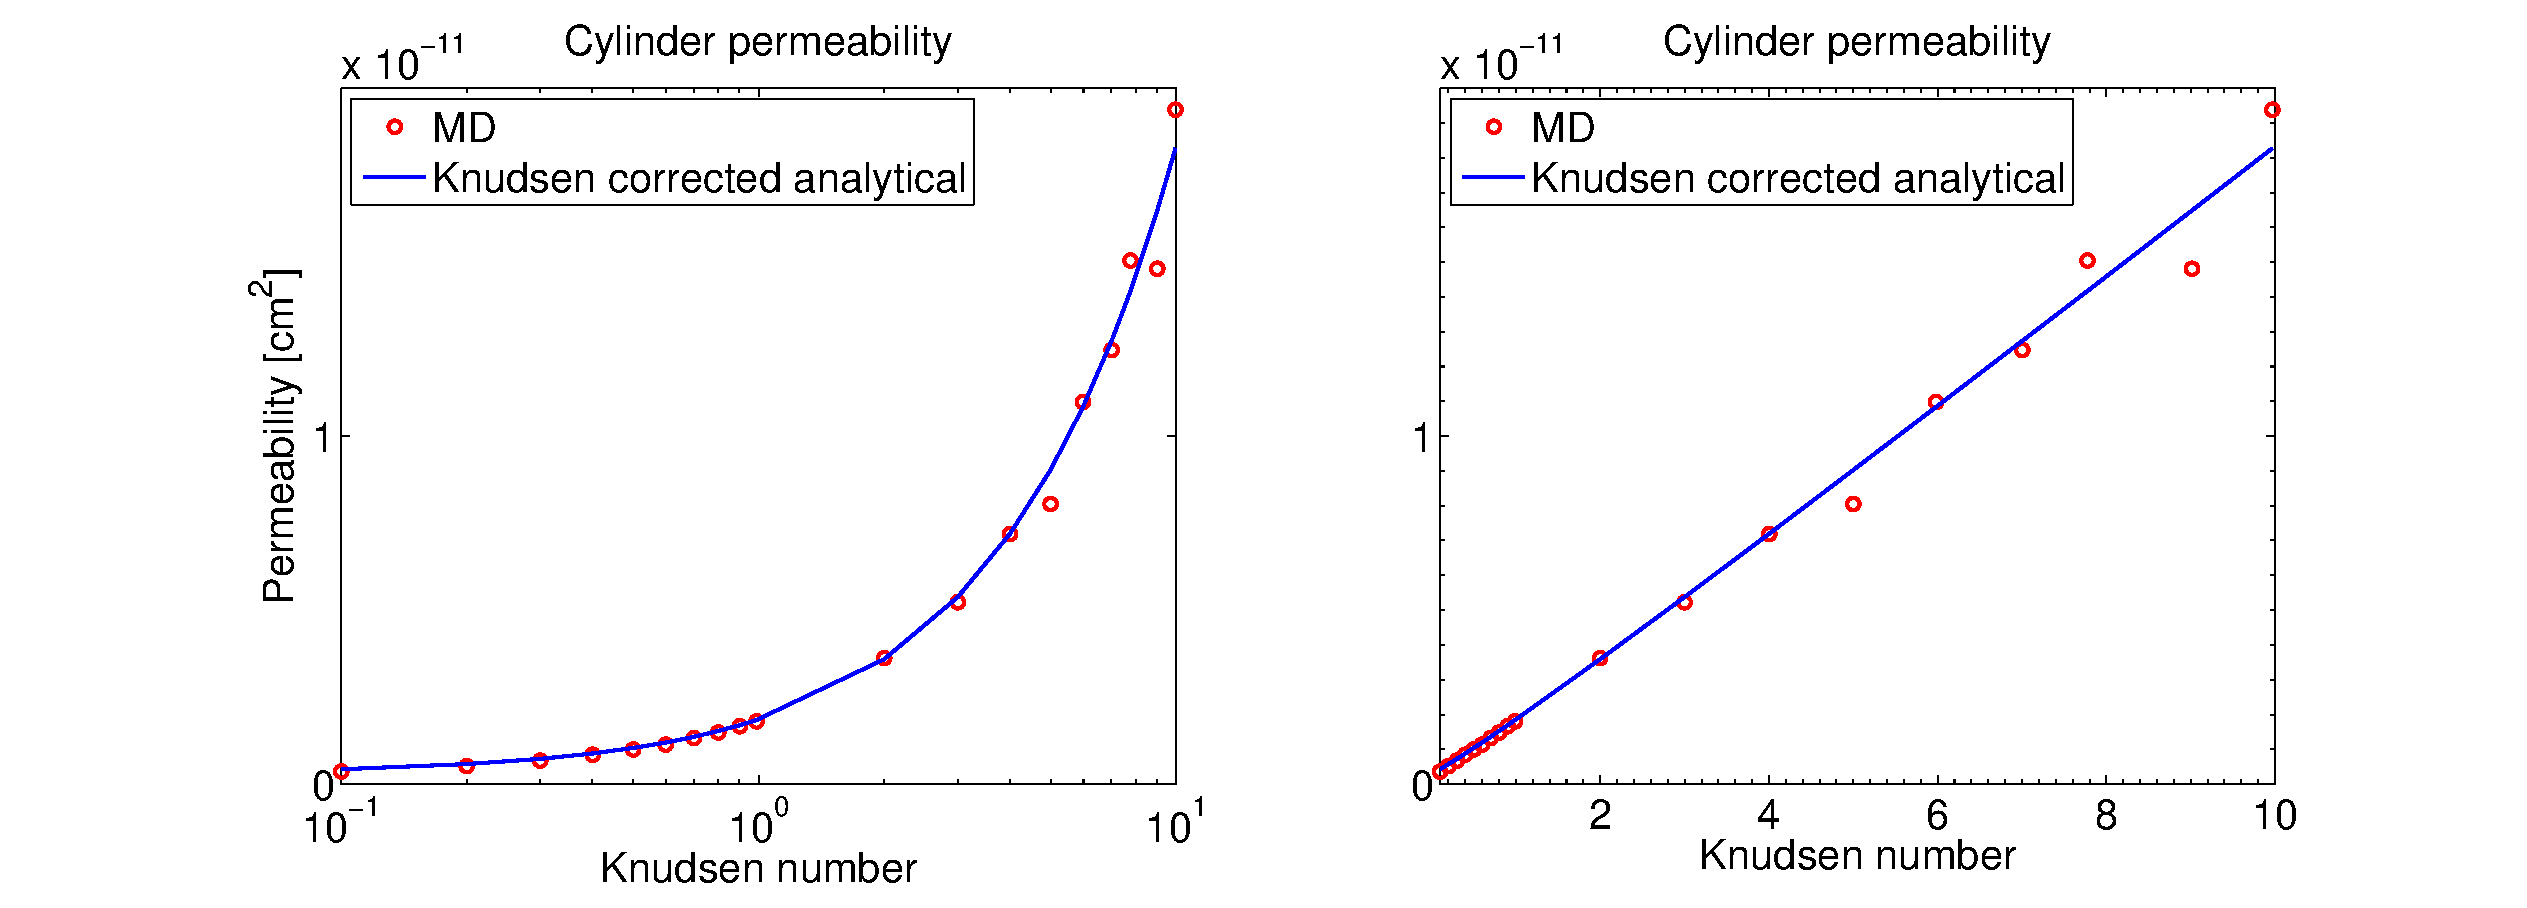
\includegraphics[width=1.0\textwidth, trim=3cm 0cm 3cm 0cm, clip]{MD/figures/permeability_cylinder.eps}
\end{center}
\caption{Permeabilitizzles fo' Knudsen numbers up in tha range $0.1$ ta $10.0$ up in a cold-ass lil cylinder wit radius $r=$\unit{151}{\angstrom}. Da left figure has a logarithmic $x-$axis ta emphasize tha phat prediction up in tha lower Knudsen range. Da right figure shows dat tha MD code produces thangs up in dis biatch accordin ta tha Knudsen erected permeabilitizzle fo' a cold-ass lil cylinder up in equation \eqref{eq:cylinder_knudsen_corrected} up in tha entire range. Da increased statistical noise is explained by dat fo' big-ass Knudsen numbers, tha number of gas atoms is low.}
\label{fig:md_permeability}
\end{figure}
  \end{chapter}  
\end{part}

\begin{part}{Visualization}
  With our newly acquired knowledge about OpenGL and learned how we can use the API to render objects on the screen, we have everything we need to develop our own visualization tools that can handle datasets from both MD and DSMC. As we now should be well aware of, the state of a system with $N$ particles is described by the $3N$ particle positions and the $3N$ velocity components. If we save this information every timestep of a simulation, we can use it to render a time series, an animation of the trajectories of all the particles. We will render the particles as spheres, but areg oing to cheat a bit. An actual sphere rendered in OpenGL would need to be composed of many triangles forming the spherical shape. To be able to render a smooth sphere, we would need more than 100 triangles \textit{per sphere} as we will see in section \ref{sec:vis_billboards}. We will apply a trick used in computer games for years. Instead of rendering spheres, we use something called \textit{billboards}, which is a rectangle with an \textit{image} (a texture) of a sphere, always pointing towards the camera. In section \ref{sec:vis_billboards}, we explain how we effectively can create and render billboards with the goemetry shader on the GPU. If the particle system has periodic symmetry (both MD and DSMC use periodic boundary conditions), we can also use the geometry shader to render copies of the system, making the illusion that the system is larger than it really is.\\
When we visualize a dataset from a DSMC simulation, we should, in addition to the particle positions, render the surface geometry (which, as we remember from section \ref{sec:dsmc_complex_geometries}, is a voxelized scalar field). We will then be able to see the surface the particles collide with which will make it easier to understand their behavior. In section \ref{sec:marching_cubes}, we discuss the so-called \textit{marching cubes} algorithm, which allows us to create a set of renderable triangles from the isosurface of a scalar field (the points where the scalar field values intersect some value).\\
We conclude the chapter by explaining how such a program was extended to render 3D images on an Oculus Rift\footnote{The Oculus Rift is a virtual reality headset displaying a stereoscopic rendering giving realistic 3D effects. The Rift has head tracking, allowing the user to tilt and rotate the head so he/she can look around in the virtual world.} in section \ref{sec:oculus_rift}. The same rendering technique was used to visualize the particles in 3D on a 3D TV.
  \begin{chapter}{OpenGL}
    \section{What is OpenGL?}
\label{sec:opengl}
OpenGL is an open source graphics library providing an application programming interface (API) to communicate with a graphics processing unit (GPU) in order to get hardware-accelerated \textit{rendering}. Rendering is the process of generating an image from \textit{models} in an \textit{environment}. These models contain information about the geometry and associated textures. A model is typically represented by a set of points, triangles or some other set of \textit{primitives}. Before discussing the model, we should explain what a primitive is.
\subsection{Primitive}
In OpenGL, the primitive decides how to interpret a set of vertices. The same set of vertices may be interpreted, hence rendered, very different on the screen. Three points can be used to draw three single points, a triangle or a part of a rectangle among other different geometries. To illustrate this idea, in figure \ref{fig:opengl_primitives}, the four vertices $\{(0,0), (0,1), (1,1), (1,0)\}$ have been rendered with the primitives \textit{GL\_POINTS}, \textit{GL\_LINES}, \textit{GL\_TRIANGLES}, \textit{GL\_QUADS} and \textit{GL\_TRIANGLE\_STRIP}. The rendered objects are of course very different depending on the primitive. 
\begin{figure}[h]
\begin{center}
\includegraphics[width=\textwidth, trim=0cm 0cm 0cm 0cm, clip]{opengl/figures/primitives.png}
\end{center}
\caption{The vertices $\{(0,0), (0,1), (1,1), (1,0)\}$ have been rendered as the primitives (from left) \textit{GL\_POINTS}, \textit{GL\_LINES}, \textit{GL\_TRIANGLES}, \textit{GL\_QUADS} and \textit{GL\_TRIANGLE\_STRIP}. We see that the final rendered geometrical objects are quite different for the different primitives.}
\label{fig:opengl_primitives}
\end{figure}
When using for example the \textit{GL\_TRIANGLES}, OpenGL interprets groups of three vertices as one triangle. In the case of \textit{GL\_QUADS}, it will of course use groups of four vertices to define the renderable object. All of the primitives (except the \textit{GL\_POINTS}) form one or more two dimensional surfaces that are colored from either the interpolated values between the vertices or from a texture map which we now will explain.
\subsection{Color interpolation}
\label{sec:opengl_color_interpolation}
When creating a primitive consisting of $N$ vertices we can color each vertex $\vec r_i$ with an RGBA vector
\begin{align}
	\vec c_i = (r_i, g_i, b_i, \alpha_i)
\end{align}
where the components are the red, green, blue and alpha values for vertex $i$. The first three components defines the color whereas the last component is the transparency. In between the $N$ vertices, there are a lot of points that do not have a defined color value. OpenGL assigns colors to these inner points by \textit{linearly interpolating} the color values of the vertices. Any point $\vec p$ in a triangle defined by the three vertices $\vec p_a, \vec p_b$ and $\vec p_c$ can be uniquely specified by using \textit{barycentric coordinates} which is a set of three numbers $(a,b,c)$ in the range $[0,1]$, normalized so that $a+b+c=1$. \todo{cite the opengl specification} Once we have these coordinates, the point $\vec p$ in the global coordinate system (in which the vertices $\vec p_i$ are defined) is found as
\begin{align}
	\vec p = a\vec p_a + b\vec p_b + c\vec p_c.
\end{align}
The barycentric coordinates are found through
\begin{align}
	a = \frac{A(\vec p, \vec p_b, \vec p_c)}{A(\vec p_a, \vec p_b, \vec p_c)}, \qquad b = \frac{A(\vec p, \vec p_a, \vec p_c)}{A(\vec p_a, \vec p_b, \vec p_c)}, \qquad c = \frac{A(\vec p, \vec p_a, \vec p_b)}{A(\vec p_a, \vec p_b, \vec p_c)}.
\end{align}
We then use the barycentric coordinates as the weights in the linear interpolation so that the color at a point $\vec p$ is given as
\begin{align}
	\vec c(\vec p) = a\vec c_a + b\vec c_b + c\vec c_c,
\end{align}
where $\vec c(\vec p_i)$ is the color we gave the vertex at $\vec p_i$. In figure \ref{fig:opengl_color_interpolation} we see how the colors are interpolated from the three values at the triangle vertices.
\begin{figure}[h]
\begin{center}
\includegraphics[width=\textwidth, trim=0cm 0cm 0cm 0cm, clip]{opengl/figures/color_interpolation.png}
\end{center}
\caption{The three vertices $\{(0,0), (1,1), (2,0)\}$ colored green, blue and red, forms a triangle where the inner points of the triangle is colored by the interpolation between the three vertices.}
\label{fig:opengl_color_interpolation}
\end{figure}
\subsection{Textures}
\label{sec:opengl_texture_interpolation}
Instead of using the colors specified per vertex, we can upload a texture (for example an image) to the graphics card so that the GPU can use that as the source of the color (this can be combined with the color values as we will see soon). The texture consists of $m\times n$ pixels where each pixel has a color $\vec c_t$. Each vertex $i$ of the triangle is assigned a \textit{local texture coordinate} 
\begin{align}
	\vec t_i = (t_x, t_y),
\end{align}
where $t_x, t_y \in [0,1]$. This gives the mapping to the \textit{global texture coordinates} (the actual pixel coordinates) $\vec t^* = (t_x^*, t_y^*)$ where 
\begin{align}
	\nonumber
	t_x^* &= m\cdot t_x\\
	t_y^* &= n\cdot t_y,
\end{align}
where we have added the asterisk on the global coordinates since we will mostly use the local ones. Since each pixel $\vec t$ (remember these are the local coordinates) in the texture has a color value $\vec c_t(\vec t)$, we can find the color $\vec c(\vec p)$ of a point $\vec p$ within the triangle by interpolating the local texture coordinates as we interpolated the colors. Remember that the point $\vec p$ has barycentric coordinates $(a,b,c)$, so the local texture coordinates $\vec t$ are found by
\begin{align}
	\vec t(\vec p) =  a\vec t_a + b\vec t_b + c\vec t_c,
\end{align}
where $\vec t_i$ is the local texture coordinate assigned to vertex $i$. The color of this point $\vec p$ is then simply
\begin{align}
	\vec c(\vec p) = \vec c_t[\vec t(\vec p)].
\end{align}
In figure \ref{fig:opengl_texture_interpolation} we have illustrated how the texture interpolation works. In the left figure, the texture is mapped with  texture coordinates corresponding to the coordinates of the triangle vertices. In the figure to the right we have a skewed mapping making the image look skewed.
\begin{figure}[h]
\begin{center}
\includegraphics[width=\textwidth, trim=0cm 0cm 0cm 0cm, clip]{opengl/figures/texture_interpolation.png}
\end{center}
\caption{Showing how texture interpolation works. Left: the three vertices $\{(0,0), (1,1), (2,0)\}$ are assigned the local texture coordinates $\{(0,0), (0.5,1), (1,0)\}$ where we see how the texture are transformed onto the triangle . Right: the three vertices $\{(0,0), (1,1), (2,0)\}$ are assigned the local texture coordinates $\{(0,0), (0,1), (1,0)\}$ where we see that the texture on the triangle is skewed because of the transformation. Note that the coordinates in the figure at the vertices are the texture coordinates, not the coordinates of the vertices.}
\label{fig:opengl_texture_interpolation}
\end{figure}
We can of course combine both these methods (colors and textures) by applying both a texture coordinate \textit{and} a color value to each vertex. OpenGL will then render an image where the rendered color $\vec C$ becomes
\begin{align}
	\label{eq:opengl_combining_colors_textures}
	\vec C(\vec p) = \vec c_t[\vec t(\vec p)] \odot \vec c(\vec p),
\end{align}
where $\odot$ is the element-wise multiplication operator defined as
\begin{align}
	(\vec a \odot \vec b)_i = a_i\cdot b_i,
\end{align}
where $\vec a,\vec b \in \mathbb{R}^N$ and $d_i$ is the $i$'th component of some vector $\vec d$. In figure \ref{fig:color_and_texture} we have combined both the color and the texture giving a triangle with the same image of Albert Einstein colored in the same way as the triangle in figure \ref{fig:opengl_color_interpolation}.
\begin{figure}[h]
\begin{center}
\includegraphics[width=\textwidth, trim=0cm 0cm 0cm 0cm, clip]{opengl/figures/color_and_texture.png}
\end{center}
\caption{We can combine both colors and textures to color points within a triangle according to equation \eqref{eq:opengl_combining_colors_textures}. Here we have used the same colors as in figure \ref{fig:opengl_color_interpolation} and the texture of Albert Einstein in figure \ref{fig:opengl_texture_interpolation}.}
\label{fig:color_and_texture}
\end{figure}
\subsection{Model}
\label{sec:opengl_model}
A model of an object contains all the information fully defining how a geometric object looks like without any effects from the environment such as light or distortions from a water surface. The model is fully described by a set $\mathcal{M}$ containing primitive objects $\mathcal{P}$, each having 
\begin{itemize}
	\item a vertex array,
	\item the primitive type,
	\item a color array,
	\item a texture id,
	\item a local texture coordinate array, and
	\item a normal vector array.
\end{itemize}
We have discussed the array of vertices, the primitive, the color and texture coordinate arrays (remember, one color and/or one texture coordinate per vertex). We also need the id (which is just an int variable) allowing us to tell the GPU which texture it should apply to this primitive object. In addition, we can assign a \textit{normal vector} to each vertex which can be used to create realistic lighting and other effects. It's time for an example of a model.\\
Say we want a model of a die. A die is a cube with six faces. The model $\mathcal M$ would then contain six primitive objects $\mathcal P_i$, each having an array of four vertices. The primitive type would be \textit{GL\_QUADS} where the color of course could be your favorite. We need to upload six textures (one face has one dot, another face has two dots etc) which gives us six different texture id's. The local texture coordinate array is simply the four corners of the unit square whereas the normal vectors should point outwards from the cube. In figure \ref{fig:opengl_die} we haved used this technique to draw a red die.
\begin{figure}[h]
\begin{center}
\includegraphics[width=\textwidth, trim=0cm 0cm 0cm 0cm, clip]{opengl/figures/die.png}
\end{center}
\caption{Drawing a die using the technique described in subsection \ref{sec:opengl_model}. The color was chosen to be red whereas each of the six faces were assigned one of the textures in the black box.}
\label{fig:opengl_die}
\end{figure}
    \input{opengl/functions}
    \section{Coordinate transformations}
\label{sec:opengl_coordinate_transformations}
OpenGL operates with three coordinate spaces that are essential to understand. 
\subsection{Model space}
\subsection{View space}
\subsection{Projection space}
    \input{opengl/textures}
    \input{opengl/shaders}
    \section{Vertex Buffer Objects}
\label{sec:opengl_vbo}
A Vertex Buffer Object (VBO) is a feature in OpenGL that allows the user to upload an array of vertices to the graphics card which can be used for very fast rendering. This could for example be a set of positions, colors or normal vectors. Once this data is uploaded to the GPU, we can render the model described by the VBO in very few function calls. We ask the GPU to give us a buffer identifier. Then we tell the GPU to allocate enough memory to store our vertices before we copy the data from the main memory to the graphics card. The data is now available on the graphics card. 
  \end{chapter}

  \begin{chapter}{Results}
    \input{opengl/marchingcubes}
  \end{chapter}
\end{part}

\begin{part}{Conclusion}
  
\end{part}
%---------------------------------------------------------------------------------------
% Appendices
%---------------------------------------------------------------------------------------
\begin{appendices}

\end{appendices}

%---------------------------------------------------------------------------------------
% Bibliography
%---------------------------------------------------------------------------------------
\printbibliography
\end{document}